\chapter{Version 1.0: Initializing the Vector (15th-Century Portugal)}
\label{ch:portugal}

\begin{tcolorbox}[colback=black!5, colframe=black!70, fonttitle=\bfseries\ttfamily, title=RUNTIME LOG: 1486 (LISBON{,} PORTUGAL)]
\ttfamily\small
\textbf{System Stress} ($\min$: class resistance): HIGH --- Domestic labor shortage threatening agricultural capital. Existing moral framework constrains exploitation of Christians.\\
\textbf{Capital} ($\max$: extraction output): STAGNANT --- Sugar trade demands labor the current moral economy cannot supply.\\
\textbf{Interference State} ($\Phi_{\text{load}}$, proximity to $\tau$): LOW axis count; phenotype partition initializing. Estimated $\Phi_{\text{load}} \in [0.10, 0.20]$, $\rho_{\tau}=M(t)/\tau \in [0.70, 0.85]$.\\
\textbf{Active Patch}: Compiling Version 1.0\ldots\\
\textbf{Variables Deployed}: The Elite Class ($E$), The Out-group ($O_{\text{racialized}}$), The In-group ($I$).\\
\textbf{Executing Function}: The Implicit Contract (Issuing the Psychological Wage).\\
\textbf{Result}: Extraction Algorithm initialized. \textbf{[POLICY]} \textit{Dum Diversas} (1452) and \textit{Romanus Pontifex} (1455) authorize unlimited exploitation. \textbf{[POLICY]} \textit{Casa dos Escravos} (1486) institutionalizes state-managed extraction. Vector established.
\end{tcolorbox}

\medskip

If we are to understand the modern mathematics of oppression, we must first examine the original source code. Systemic racism constituted a calculated, mathematical technology engineered by an Elite class to solve a specific economic problem.

To find the compilation date of this algorithm, we must look to 15th-century Portugal. The Portuguese Crown---the Elite---was expanding its global empire, driven by the highly lucrative sugar trade. The Elite faced a severe system stressor: a shortage of cheap domestic labor to work the plantations. To scale their capital, they needed a new class of labor that could be extracted indefinitely, free of wages, rights, and the threat of peasant revolts.

Workers alone would not suffice. The Elite needed to \textbf{bifurcate the human population} and simultaneously mint two new variables: the Out-group and the In-group.

This is the first literal installation of the fractal mind virus. The Portuguese Crown captured bodies while writing a predictive rule into the social world: African meant extractable, Christian-European meant protected, and the difference could be treated as visible before any individual act was known. Once that rule entered law, liturgy, trade paperwork, and ordinary perception, the virus no longer needed every host to understand the economic objective. It only needed the host wetware to run the racial prior automatically.

\subsection{The Vector Equation of Racism}

Traditional sociological models frequently err by calculating prejudice as a \textit{scalar} quantity. In mathematics and physics, a scalar is a metric possessing magnitude but lacking a definitive direction (like temperature or speed). An individual's personal bias or anger is a scalar---emotional weight, but it lacks the institutional momentum to alter society.

Under the strict parameters of the mathematics of oppression, systemic racism cannot be a scalar. It must be defined as a \textbf{vector}. A vector possesses both magnitude \textit{and} a specific, irreversible direction. The foundational insight that racism operates as a directional force was articulated by Palestinian-American author and activist Susan Abulhawa, who framed the distinction between racism as mere prejudice and racism as a state-directed vector in an interview on the Bad Faith Podcast \cite{abulhawa}. The formalization developed in this book---specifying the magnitude term $M$, the directional forcing term $\hat{d}_{\text{state}}$, and their relationship to the Predatory Min-Max Function---extends and mathematizes that foundational framing.

\begin{equation}\label{eq:2.1-racism-vector}
\vec{R}_{\text{acism}} = M_{\text{agnitude}} \cdot \hat{d}_{\text{state}}
\end{equation}

\noindent\textit{Note on formalization.}\footnote{This equation is classified as Tier~3 (ordinal/structural); the directional decomposition is a conceptual formalization establishing the scalar-vs-vector distinction. The state-power direction $\hat{d}_{\text{state}}$ is validated by the historical sequence of deliberate Elite design documented in this chapter. See the Empirical Methodology chapter (p.~\pageref{ch:empirical_methodology}) and Appendix~\ref{app:empirical_index}.} This equation is a \textbf{conceptual formalization}---a pedagogical device for establishing the scalar-vs-vector distinction and for making precise that individual prejudice ($M$, a scalar) produces systemic racism only when combined with the state-supplied directional force ($\hat{d}_{\text{state}}$). It does not specify a vector space or basis vectors, and is not intended to function as a quantitative predictive formula. The full mathematical apparatus---including the precise specification of extraction flows, suppression dynamics, and directional forcing---is carried by the Predatory Min-Max Function and the phase-loading engine introduced in Chapter~1. Consistently with the diagnostic model developed there (Section~1.2), this book reserves the term \textit{racism} for the directed institutional vector; phenotypic bias, prejudice, and pre-vector dehumanization are treated as components of $M$---necessary inputs that cannot produce systemic racism without $\hat{d}_{\text{state}}$.

In this equation, $M$ represents the magnitude of human prejudice. The true engine of the equation is $\hat{d}_{\text{state}}$---the top-down directional force provided by the state.

The Portuguese Elite engineered this vector through a dual-authorization mechanism. First, they secured the moral architecture via the Catholic Church (such as the 1452 Papal Bull \textit{Dum Diversas}) \cite{dumdiversas}. Second, they built the legal infrastructure, establishing the \textit{Casa dos Escravos} (House of Slaves) in Lisbon in 1486. By royal decree, all enslaved Africans had to be processed and taxed through this specific state customs house. The Elite provided the directional force ($\hat{d}_{\text{state}}$) that transformed baseline xenophobia into a state-managed, highly profitable extraction machine.

\section{Portuguese Class Dynamics and the Elite's Dilemma}

Before understanding the invention of race, we must first understand the class dynamics that necessitated it. In 15th century Portugal, as in much of medieval Europe, society had achieved a degree of class solidarity that constrained Elite exploitation. The feudal system, while hierarchical, operated within a shared moral framework: all humans, regardless of status, were part of the same moral community. Peasants and nobility alike were Christians, subjects of the same crown, and---significantly---recognized as human beings with souls.

This moral inclusion created practical limits on exploitation. The Elite extracted labor through serfdom and taxation under specific constraints:
\begin{itemize}
    \item \textbf{Religious doctrine}: The Catholic Church, despite supporting hierarchy, imposed limits on the treatment of Christians. Enslavement of fellow Christians was prohibited or heavily restricted.
    \item \textbf{Legal protections}: Even serfs had some legal standing---they could not be killed arbitrarily, families could not be separated at will, and certain customary rights were recognized.
    \item \textbf{Social cohesion}: Shared identity as Portuguese, as Christians, and as humans created bonds that could translate into solidarity against Elite overreach.
    \item \textbf{Demographic limits}: The available labor pool consisted of people who belonged to the moral community, limiting how brutally they could be exploited without risking rebellion or moral condemnation.
\end{itemize}

The Portuguese Elite faced a fundamental problem: \textbf{how to create a permanent slave class without violating the moral framework that constrained exploitation of the existing population}. They needed a labor force that could be worked to death, families that could be separated, and people who could be treated as property---all without triggering the moral and legal protections that applied to humans.

In solving this, the Elite did not invent the concept of identifiability from a vacuum. Two pre-existing precedents supplied the raw material.

The first was the European subjugation of women. This predates the invention of modern racial capitalism and provided the foundational architectural template for extracting labor through the enforcement of an easily identifiable biological boundary. Women, as a historically subjugated class within Europe, already existed as a population whose autonomy was restricted based on immutable, visible characteristics. The Elite recognized that the efficacy of an Out-group partition depends on the \textit{speed and certainty of identification}. By adapting the pre-existing logic of gendered subjugation to the axis of skin color, the Elite were able to scale the extraction algorithm to encompass entire populations, ensuring that the racialized Out-group could never blend back into the moral community.

The second was the Islamic trans-Saharan slave trade. Centuries before the first Portuguese caravel reached West Africa, Arab and Berber merchants had operated documented trade routes moving enslaved sub-Saharan Africans across the Sahara to the Mediterranean and Middle East---a system historians estimate transported upward of eight million people between the 7th and 15th centuries \cite{lewis_race}. The theological justification was already in place: medieval Islamic scholars had reinterpreted the Curse of Ham (Genesis 9:25) to classify sub-Saharan Africans as the cursed descendants of Noah's son Ham, condemned by divine decree to perpetual servitude---a doctrine deployed as cover for a commercial enterprise whose scale was staggering. The Zanj, enslaved East Africans put to plantation-scale labor in the marshlands of the Abbasid Caliphate near Basra, staged the largest slave revolt of the medieval world, a fourteen-year insurrection (869--883~CE) that required the full military mobilization of the Caliphate to suppress \cite{popovic_zanj}. The revolt failed; the trade continued. The Curse of Ham doctrine and the phenotypic partition it rationalized were already operational centuries before Zurara set pen to parchment.

The Portuguese Elite inherited phenotypic prejudice against sub-Saharan Africans and gave it an \textbf{industrialized global architecture}: the first legal and commercial system to transform locally deployed phenotypic prejudice into a self-replicating, transnationally enforceable, legally codified racial capitalism. The Curse of Ham pre-existed Zurara. The \textit{Casa dos Escravos}, the papal bulls authorizing unlimited enslavement, the \textit{partus sequitur ventrem} supply-chain statute, the insurance markets built on enslaved bodies as cargo, and the One Drop Rule did not. That is the zero-day: prejudice compiled into a permanent, heritable, globally exportable operating system.

This architectural distinction---between pre-existing prejudice and its institutionalized global compilation---receives independent corroboration from institutional economics. Acemoglu and Robinson's canonical study of why nations fail identifies the Portuguese Atlantic system as the textbook inauguration of \textit{extractive institutions}: legal and economic arrangements designed to concentrate wealth at the apex of a hierarchy rather than to generate broad-based prosperity \cite{acemoglu_robinson}. Their analysis confirms the framework's zero-day claim at the level of comparative political economy. AJR's model is structurally incomplete for the purposes of this book: it lacks the racial-partition variable ($I_{\text{buffer}}$ vs.\ $O_{\text{racialized}}$) and the psychological wage ($\psi$) that explain \textit{why} extractive institutions in racialized systems become self-perpetuating in a way that mere inefficiency cannot explain---and why every subsequent ``inclusive'' reform is absorbed without dismantling the kernel. That critique is developed fully in Section~\ref{sec:acemoglu_limit}.

The solution was elegant and horrifying: \textbf{remove an entire category of people from the moral community by reclassifying them as subhuman property}.
\section{The Invention of Race as Moral Exclusion}

The concept of race and the systemic nature of racism have their roots deeply embedded in this Elite need to break class solidarity and create a slave class unconstrained by moral limits. A pivotal figure in this narrative is Gomes de Zurara, whose work in the 1450s laid the groundwork for the racialization of African peoples. Commissioned by the Portuguese monarchy, Zurara authored a chronicle that justified the enslavement of African individuals by portraying them as a monolithic group, inherently inferior and \textit{subhuman} \cite{zurara, kendi}. 

This was \textbf{ontological exclusion}. Zurara's narrative went beyond claims of inferiority and positioned Africans as \textit{a separate species}, more akin to animals than people. This act of lumping together the diverse peoples of Africa into a single, derogatory category represented an unprecedented move towards institutionalizing race as a basis for systemic oppression.

Dr.\ Ibram X.\ Kendi highlights Zurara's role in inventing race and racism, noting that his descriptions were instrumental in justifying the Portuguese slave trade \cite{kendi}. Zurara's narrative supplied moral and intellectual justification for the kidnapping and enslavement of African people while setting a precedent for European engagement with sub-Saharan Africa. Portugal, thus, became the first European nation to sail directly to sub-Saharan Africa for the purpose of capturing human beings for enslavement.

\subsection{The Kidnapping Operations: What Zurara Actually Documented}

The conventional framing of the early slave trade as ``trade'' obscures its operational reality. The Portuguese did not begin by trading with West African kingdoms. They began by \textbf{kidnapping}. Zurara's own chronicle---the same text that invented the racial justification---is simultaneously the operational log of armed raiding expeditions.

On August 8, 1444, a fleet of six ships organized by the \textit{Companhia de Lagos} and led by Lançarote de Freitas returned to Lagos, Portugal, carrying 235 kidnapped people---Sanhaja Berbers seized in pre-dawn raids on the islands and coastal settlements of Arguin Bay (modern-day Mauritania). The captives were paraded to an open field outside the city walls and partitioned into lots for sale in the presence of Prince Henry the Navigator, who collected the royal fifth and knighted Lançarote on the spot. Zurara, who witnessed the event, recorded the scene: families torn apart, mothers clutching children, captives collapsing on the ground---and then proceeded to frame the atrocity as a divinely sanctioned deliverance of souls from paganism.

The subsequent 1445--1446 expedition, a larger fleet of fourteen ships, pushed south toward the Wolof lands of modern-day Senegal. There the Portuguese encountered organized military resistance---the Wolof repelled raiding parties and attacked negotiators---demonstrating that the earliest phase of the slave trade was not a commercial exchange between willing parties but an \textit{armed invasion} met with armed resistance. The Portuguese succeeded only where their firearms and naval superiority allowed them to overwhelm coastal settlements before defenders could organize. Where resistance was effective, the raiders retreated.

The transition from raiding to ``trading'' was itself a function of the arms asymmetry documented in Chapter~\ref{ch:kinetic}. Direct kidnapping became logistically costly as coastal populations mobilized defensive responses. The Portuguese shifted to a more efficient extraction model: selling firearms to coastal kingdoms and accepting enslaved human beings as the only currency---creating the exponential feedback loop (Section~9.1.2) that would eventually consume the continent.

This shift is sometimes raised as a challenge to the elite-design thesis: if African kingdoms---Kongo, Benin, and later Dahomey and Asante---actively participated by supplying war captives, does that not complicate the picture of Portuguese unilateral moral engineering? It confirms the algorithm's most important structural property: \textbf{modularity}. The Portuguese extraction system required only a sufficiently attractive exchange rate to recruit local elites into the supply chain. African kingdoms that participated did so through their \textit{own} pre-existing elite extraction logic---captives from warfare were already a resource within African political economies, and firearms were a transformative military asset. The Portuguese algorithm did not override African elite agency; it \textit{interfaced} with it, converting a regional phenomenon into a transatlantic one by offering an exchange that local elites found rational at the point of transaction. The moral-exclusion architecture was applied at the destination, not the source: the ontological reclassification of Africans as subhuman property was the Portuguese legal innovation, imposed in Lisbon, Madeira, and later Virginia---not something African kingdoms were asked to internalize or endorse. That African elites sold captives into a system whose full downstream logic they did not control is precisely what makes the algorithm dangerous: it recruits participants at each node through locally legible incentives while reserving the system-level moral hack for the architects. The origin point was not trade. It was armed kidnapping, documented by the same chronicler who invented the racial justification for it.

The populations subjected to this algorithm diagnosed it in real time. Woodard recovers the African counter-archive---spanning Bakongo, Igbo, Fanti, and Bornu peoples---which recognized the European extraction kernel as literal cannibalism, rejecting the framing of a civilizing mission. In 1818, Ali Eisami (a Bornu captive) documented the terror of the Middle Passage: the white minister who ``took hold of my hand, and drew me into his house,'' the whispered rumor that ``the White man has taken Ali \dots to slaughter him,'' the imagined long knife \cite{curtin_africa}. The European deployment of the ``savage African cannibal'' stereotype was therefore a documented instance of projection---the actually-cannibalistic extraction kernel attributed its own operative behavior to its victims, thereby masking the algorithm behind a counter-accusation. This is the earliest instantiation of $P_{\text{gaslight}}$: the system hides its consumption of the Out-group by accusing the Out-group of being the consumers \cite{woodard_delectable}.

\section{The Original Implicit Contract and the Psychological Wage}
\label{sec:dubois_wage}

Minting the Out-group solved the Elite's labor shortage, but it introduced a secondary vulnerability. The Portuguese Elite still had to manage their own impoverished, starving peasant class. If the working class realized that the Elite were hoarding all the wealth generated by this new extraction model, the system could crash via a populist revolt.

To stabilize the system, the Elite executed a psychological patch: the \textbf{Original Implicit Contract}.

You cannot mathematically define an Out-group without simultaneously creating an \textbf{In-group}. By legally defining the Out-group as subhuman commodities through the \textit{Casa dos Escravos}, the Elite automatically established the In-group ($I$)---their own peasantry---as the permanent, artificial floor of humanity.

\begin{quote}
\textit{``You may be poor, you may be exploited, but you will never be slaves. Your children will never be slaves. We do not enslave humans, and these Africans are not human---they are a subspecies, no different from cattle. Therefore, there is no reason not to exploit their labor, and your humanity is secured by their exclusion from humanity.''}
\end{quote}

The Elite compensated the In-group with a \textbf{suppression allocation} ($\psi$), which required no redistribution of physical wealth or capital from $E$. Following W.E.B.\ Du~Bois \cite{dubois}, who identified this mechanism in *Black Reconstruction in America* (1935) as a ``\textbf{public and psychological wage}''---a compound of social status \textit{and} public infrastructure advantages---this framework formalizes $\psi$ as a two-mode variable and traces it to its 15th-century origins, predating Du Bois's Reconstruction-era analysis by four centuries. The mathematical function of the contract is:

\begin{equation}\label{eq:2.2-status-suppression-allocation}
S_{\text{tatus}}(I) = \text{Base\_Humanity} + \psi(t), \quad \psi(t) = \psi_s(t) + \psi_m(t)
\end{equation}
\begin{equation}\label{eq:2.3-psi-null-in-survival}
S_{\text{tatus}}(I) > S_{\text{tatus}}(O_{\text{racialized}})
\end{equation}

where\footnote{Equations~\ref{eq:2.2-status-suppression-allocation}--\ref{eq:2.3-psi-null-in-survival} are classified as Tier~3 (ordinal/structural). Equation~\ref{eq:2.2-status-suppression-allocation} formalizes Du Bois's ``public and psychological wage'' \cite{dubois}; the structural claim that $\psi_m(t)$ is activated only under kinetic threat is validated by the 1705 Virginia Slave Codes and New Deal racially partitioned benefits documented in Chapter~\ref{ch:bacon}. Equation~\ref{eq:2.3-psi-null-in-survival} is a structural ordering whose ordinal direction is confirmed by the documented history of differential legal status---from the \textit{Casa dos Escravos} (1486) through \textit{Dred Scott} (1857)---correlating with kinetic-threat levels. See the Empirical Methodology chapter (p.~\pageref{ch:empirical_methodology}) and Appendix~\ref{app:empirical_index}.} $\psi_s(t)$ is the \textbf{status wage}---the non-material guarantee of ontological superiority, deference, and racial privilege---and $\psi_m(t) \geq 0$ is the \textbf{material wage}, deployed only when class-coherence threat $M(t)$ approaches the critical threshold $\tau$. $\psi_m(t)$ is never sourced from $E$'s own extraction; it is always funded by \textit{increasing extraction from $O_{\text{racialized}}$}, preserving the invariant $\Delta\max = 0$.

\subsubsection{The Electrodynamic Reframing: $\psi$ as Complex Power}

The scalar addition $\psi = \psi_s + \psi_m$ captures the magnitude of the
suppression allocation but obscures its \textbf{structure}. In the Unified
Electrodynamic Framework (Chapter~\ref{ch:system_init},
Eq.~\ref{eq:0.1-unified-lorentz-force}), the suppression allocation is not a
scalar sum but a \textbf{complex number}:
\begin{equation}\label{eq:2.2a-complex-suppression-allocation}
W = \psi_m + j\psi_s
\end{equation}
where $j = \sqrt{-1}$ signals that $\psi_s$ operates in a domain
\emph{orthogonal} to material reality. The relation follows the exact
mapping used in electrical engineering to distinguish \textbf{real power}
(Watts, performs physical work) from \textbf{reactive power} (VARs, sustains the
field but does zero work).

\begin{definition}[Complex Suppression Allocation $W$]
\label{def:complex-wage}
The Complex Suppression Allocation is:
\begin{equation}\label{eq:2.2b-complex-wage-def}
W = \psi_m + j\psi_s
\end{equation}
\begin{itemize}
    \item $\psi_m \in \mathbb{R}$: the \textbf{Material Wage}---real economic
    concessions (land, capital, healthcare) that perform actual physical work on
    the Buffer Class. Sourced from deeper $O_{\text{racialized}}$ extraction.
    \item $j\psi_s \in j\mathbb{R}$: the \textbf{Psychological/Status
    Wage}---the non-material guarantee of ontological superiority. Costs $E$
    zero capital. Operates as reactive power: it deflects class momentum without
    transferring material energy.
\end{itemize}
In polar form:
\begin{equation}\label{eq:2.2c-polar-form}
W = R \angle\theta = R e^{j\theta}, \quad R = |W| = \sqrt{\psi_m^2 + \psi_s^2}
\end{equation}
where $\theta$ is the \textbf{phase angle} of oppression.
\end{definition}

The phase angle $\theta$ diagnoses the system's operating mode:
\begin{itemize}
    \item $\theta = 0°$: Wage is 100\% material. The Buffer Class receives genuine
    economic investment (e.g., strong social democracy, massive public works).
    \item $\theta = 90°$: Wage is 100\% psychological. Zero material benefit;
    complete pacification through symbolic status superiority. This is the
    \textbf{default operating mode} of the extraction kernel.
    \item $\theta > 90°$ (Quadrant~II): $\cos\theta < 0$. The Elite is actively
    extracting material wealth \emph{from} the Buffer Class while feeding
    hyper-inflated psychological wages. \textbf{This is the mathematical
    definition of fascism within the framework.}
\end{itemize}

\begin{theorem}[Imaginary Squaring as Material Destruction]
\label{thm:imaginary-squaring}
If a Buffer Class individual or polity over-indexes exclusively on the
psychological wage (let $W = j\psi_s$, pure imaginary), then squaring this
allocation yields:
\begin{equation}\label{eq:2.2d-imaginary-squaring}
(j\psi_s)^2 = j^2 \psi_s^2 = -\psi_s^2
\end{equation}
The result is a \emph{negative real number}. Compounding purely symbolic status
wages destroys real material wealth. This provides a rigorous mathematical proof
of the mechanism by which the Buffer Class votes against its own healthcare,
unions, and infrastructure to maximize racial or cultural status.
\end{theorem}

\begin{theorem}[Solidarity as Imaginary Cancellation]
\label{thm:solidarity-cancellation}
If the Elite's wage is $W = \psi_m + j\psi_s$, the \textbf{complex conjugate}
is $W^* = \psi_m - j\psi_s$, representing the revolutionary rejection of the
psychological wage. When the Buffer Class adopts $W^*$ and aligns with the
Out-group:
\begin{equation}\label{eq:2.2e-solidarity-addition}
W + W^* = (\psi_m + j\psi_s) + (\psi_m - j\psi_s) = 2\psi_m
\end{equation}
The imaginary status wage cancels entirely. Real material power doubles. The
horizontal deflection collapses; combined class momentum is now purely vertical,
directed at the Elite.
\end{theorem}

These theorems explain why the Elite is existentially threatened by cross-group
class solidarity: the mathematics guarantee that rejection of the imaginary axis
removes all horizontal deflection and amplifies real material force against the
extraction kernel.

The contract dictated that no matter how destitute, hungry, or exploited the In-group peasant was, they retained the exclusive legal status of ``human.'' They could not be commodified or legally processed as property.

In its inaugural Portuguese deployment, $\psi_m = 0$: the Elite pacified their working class without spending a single coin, buying their loyalty entirely through the distribution of \textit{optical superiority}. The In-group accepted their economic subjugation because the system guaranteed them social supremacy over the Out-group. Later deployments---the 1705 Virginia Slave Codes, the New Deal's racially partitioned benefits---would activate $\psi_m > 0$ when status wages alone proved insufficient to hold $\min$ below $\tau$.

A structurally important question follows from the geography: if the enslaved population was held offshore---on Madeira's sugar estates, in S\~{a}o Tom\'{e}, and later in Brazil---how did the psychological wage reach Portuguese peasants who would never see an enslaved African in a Lisbon street? The answer is that $\psi_s$ requires only that the legal partition be \textit{legible} to the In-group; physical co-presence is unnecessary. The \textit{Casa dos Escravos} generated official registries classifying Africans as property rather than persons---documents that circulated through the Crown's administrative apparatus and were enforced in every Portuguese port, customs house, and notary office. Zurara's chronicle, commissioned by the Crown and read aloud in court, published the ontological exclusion as official narrative. Royal proclamations defined the enslaved as a legally distinct category of being whose children would inherit the same status. A Portuguese peasant did not need to stand next to an enslaved African to receive the status wage; they needed only to exist within a legal order that classified one group as human and another as taxable cargo. This is the mechanism's general form: the psychological wage is transmitted through \textit{institutional legibility}; proximity is unnecessary. The later American deployment---where plantation co-labor \textit{did} place white servants and enslaved Africans side by side---differed from the Portuguese norm. It was the stress test, the edge case that nearly broke the system (Chapter~\ref{ch:bacon}). The Portuguese version demonstrated that the wage can be issued and received entirely through law, language, and the administrative record.

\begin{definition}[Slave Capitalism]
\textbf{Slave capitalism}: a distinct economic model that combines capitalist accumulation with racialized slave labor, in which the Elite secures working-class complicity through an implicit contract that offers racial status in exchange for tolerating---and enforcing---the ontological exclusion of an enslaved population from the moral community.
\end{definition}

This contract accomplished several objectives for the Elite:

\begin{enumerate}
    \item \textbf{Broke class solidarity}: Portuguese workers could no longer identify with enslaved Africans as fellow laborers because Africans were defined as non-human. Any solidarity based on shared exploitation was severed by the ontological divide.
    
    \item \textbf{Created psychological compensation}: Material improvement played no role; poor Portuguese gained status through racial categorization. The ``wages of whiteness'' (though the term would emerge later) began here: your poverty matters less when you are assured you belong to the human race and others do not.
    
    \item \textbf{Eliminated moral constraints}: By removing Africans from the moral community, the Elite eliminated the religious, legal, and social protections that constrained exploitation. Africans could be worked to death, families could be torn apart, children could be sold---none of the protections afforded to humans applied.
    
    \item \textbf{Secured labor expansion}: The Elite gained access to a theoretically unlimited labor supply that could be brutally exploited without triggering the moral frameworks that protected Portuguese workers.
    
    \item \textbf{Prevented future solidarity}: The racial framework ensured that even if African-descended peoples gained freedom, the ontological divide would persist, preventing alliances between exploited groups across racial lines.
\end{enumerate}

The model proved extraordinarily profitable for the Elite class, generating wealth accumulation at scales previously impossible under feudalism or wage labor systems \cite{williams, robinson}. The Implicit Contract and its psychological wage would be replicated wherever the algorithm was exported---across the Atlantic to the Americas, and eventually across the entire colonial world. The enforcement apparatus, the geographic displacement, and the modern continuity of this slave capitalism will be traced in their proper chronological positions as the algorithm iterates through its subsequent versions.

\subsection{The Roman Control Case: Slavery Without Racial Coding}

The claim that the Portuguese Elite \textit{invented} the racial partition---that racial coding was an engineered addition to slavery---requires a control case. The Roman Empire provides it.

Rome operated one of history's largest slave economies for over seven centuries. At its peak, an estimated 10--20\% of the population---between 5 and 15 million people---were enslaved. Slaves powered the \textit{latifundia} (vast agricultural estates), maintained the aqueduct and sewer systems, served as teachers, accountants, physicians, and scribes, and were bought and sold at auction as chattel property. By any structural definition, Roman slavery was a fully operational extraction kernel: $\max \mathcal{E} - \min(O_{\text{slave}})$.

But the Roman kernel lacked the variable that defines the American system. Roman slaves were drawn from every ethnicity the Empire conquered: Gauls, Germans, Greeks, Syrians, Britons, Egyptians, Judeans, North Africans. The membership function for the enslaved class was:

\begin{equation}\label{eq:2.4-roman-membership-function}
O_{\text{slave}}^{\text{Roman}} = f(\text{conquest}, \text{debt}, \text{crime}, \text{birth})
\end{equation}

This\footnote{This equation is classified as Tier~3 (ordinal/structural); the multi-ethnic and permeable composition of Roman slavery is documented by Bradley's \textit{Slavery and Society at Rome} \cite{bradley_slavery_rome} and serves as the control-case baseline for isolating the American phenotypic innovation. See the Empirical Methodology chapter (p.~\pageref{ch:empirical_methodology}) and Appendix~\ref{app:empirical_index}.} function was \textit{permeable} and \textit{non-heritable in principle}. A Roman slave could purchase freedom through the \textit{peculium} (a personal fund the law allowed them to accumulate). Manumission was common enough that an estimated 20\% of urban slaves achieved it. Freedmen could amass wealth, manage businesses, and---significantly---their \textit{children could hold political office}. The Roman Senate once considered requiring slaves to wear distinctive clothing but abandoned the proposal for fear that ``slaves would realize their numbers and rebel''---an acknowledgment that the enslaved population was phenotypically indistinguishable from the free poor.

Compare this to the American function the Portuguese invented and the Virginia Elite codified:

\begin{equation}\label{eq:2.5-american-racial-function}
O_{\text{racialized}}^{\text{American}} = f(\text{phenotype})
\end{equation}

This\footnote{This equation is classified as Tier~3 (ordinal/structural); the permanent and heritable phenotypic lock is documented by the 1662 Virginia \textit{partus sequitur ventrem} statute (Hening's \textit{Statutes at Large}, Vol.~II) and confirmed across 195 years through \textit{Dred Scott} (1857) \cite{dredscott}. See the Empirical Methodology chapter (p.~\pageref{ch:empirical_methodology}) and Appendix~\ref{app:empirical_index}.} function was \textit{permanent}, \textit{heritable}, and \textit{sealed}. No amount of labor, talent, or wealth could alter the membership criterion. The 1662 Virginia law of \textit{partus sequitur ventrem} (``the child follows the mother'') ensured that the enslaved class was self-reproducing and inescapable. Freedmen's children remained racially coded and subject to re-enslavement or exclusion. The 1857 \textit{Dred Scott} decision confirmed what the system had encoded from the beginning: persons of African descent ``had no rights which the white man was bound to respect.'' \cite{dredscott}

The Roman comparison isolates the variable. Both systems ran the extraction kernel. Both systems commodified human beings, subjected them to lethal violence, and generated Elite wealth through forced labor. But only the American system locked the enslaved class to a \textit{phenotypic marker} that survived manumission, survived generational passage, and survived even the formal abolition of slavery itself. The racial partition is the specific innovation that the Portuguese Elite introduced in the 1440s and the Virginia Elite formalized in 1705. Rome proves that the extraction kernel can operate without it---which means that everywhere the racial partition appears in the American system, it was \textit{put there by design}.

\subsection{The Religious Partition: Pre-Racial Ideological Justification}

The Roman control case demonstrates that the extraction kernel can operate without racial coding. A second control case demonstrates something equally important: the \textit{partitioning strategy itself} predates race. Before the Portuguese invented the racial Out-group in the 1440s, the European Elite had already perfected the technique of splitting populations along ideological fault lines---using religion as the partition variable.

The French Wars of Religion (1562--1598) killed an estimated 3 million people. The St.\ Bartholomew's Day Massacre of 1572 alone saw Catholic mobs, incited by the Crown, slaughter between 5,000 and 30,000 Huguenot Protestants across France in a matter of weeks. The structural logic is identical to the racial partition: the Elite ($E$) designated a subpopulation as the ideological Out-group ($O_{\text{religious}}$), justified their exclusion through spurious theological claims ($J_{\text{religious}}$), and deployed the co-religionist majority as a Buffer Class ($I_{\text{Catholic}}$) to enforce the boundary through violence. The Huguenots were French citizens---neighbors, colleagues, family members---reclassified as existential threats through an act of ideological partitioning.

The Thirty Years' War (1618--1648) scaled this logic to the continental level, killing an estimated 8 million people---roughly 20\% of the German-speaking population. What began as a conflict between Catholic and Protestant states in the Holy Roman Empire became the deadliest European conflict before the twentieth century. The extraction function operated through the same architecture: Elite factions used religious identity to mobilize populations against each other, while the material consequences---famine, displacement, demographic collapse---fell exclusively on the peasant and working classes who constituted the actual combatants. The Peace of Westphalia (1648), which ended the war, froze the partition into territorial boundaries, leaving the underlying extraction dynamic intact and allowing each Elite faction to monopolize extraction within its own domain.

The structural parallel is precise:
\begin{equation}\label{eq:2.6-roman-american-structural-parallel}
O_{\text{religious}}^{\text{pre-1450}} = f(\text{doctrine, sect, heresy}) \quad \longrightarrow \quad O_{\text{racialized}}^{\text{post-1450}} = f(\text{phenotype})
\end{equation}

The\footnote{This equation is classified as Tier~3 (ordinal/structural); the structural mapping from religious to racial partition is an analogy documenting variable substitution, not a claim of phenomenological equivalence between the French Wars of Religion and the Atlantic slave trade. The parallel is validated by the documented architectural sequence in this chapter. See the Empirical Methodology chapter (p.~\pageref{ch:empirical_methodology}) and Appendix~\ref{app:empirical_index}.} Portuguese innovation was the discovery that \textit{phenotype} was a superior partition variable to \textit{religion}. Ideological partitioning itself predated the Portuguese; the function changed its input variable while the output---a partitioned population with one segment designated for exclusion, exploitation, and violence---remained identical.

\subsection{The Irrelevance of Phenotype: Variable-Based vs. Identity-Based Analysis}

A necessary conceptual leap required by this framework is the transition from an \textit{identity-based} analysis of racism to a \textbf{variable-based (or role-based) analysis}.

Traditional anti-racist discourse often assumes the system is driven by an essential, irrational hatred of a specific identity group (e.g., ``white people inherently hate Black people''). The mathematical framework rejects this. The system is fundamentally \textbf{identity-agnostic}. It targets phenotype because phenotype supplies the most efficient, zero-cost \textit{sorting key} for its extraction algorithm. Irrational hatred is not the operating variable.

The roles within the Predatory Min-Max Function---the Advantaged ($I_{\text{buffer}}$) and the Disadvantaged ($O_{\text{racialized}}$)---are structural positions. While historically and empirically these positions have been filled based on race, the \textit{structure itself} does not care about the identity of the occupants. 

This variable-based understanding neutralizes the most common defense mechanism of the Buffer Class: ``I am not a racist; I don't harbor hatred in my heart.'' Under the set-theoretic model, personal hatred is entirely irrelevant. The relevant question is whether one occupies the structural role of the Buffer Class ($I_{\text{buffer}}$), receives the psychological wage ($\psi$), and enforces the extraction kernel. Personal hatred is irrelevant to the structural diagnosis.

If the mathematical requirements of the extraction engine changed tomorrow, the Elite ($E$) would instantly rewrite the sorting algorithm to partition the population by religion, political affiliation, or genetic bio-markers. The suffering of the Out-group follows from their assigned variable within the extraction equation; identity itself supplies no explanatory force.

The decisive advantage was \textbf{identifiability}. Under religious partitioning, the Out-group was \textit{invisible by default}.
 A Huguenot walking through a Catholic quarter looked identical to every other Frenchman. A crypto-Jew in Inquisition-era Spain could attend Mass, recite the correct prayers, and pass undetected for generations. The system required elaborate surveillance infrastructure to function: loyalty oaths, informant networks, forced public confessions, distinctive clothing mandates (the \textit{sanbenito}, the yellow badge). Even with this apparatus, the boundary leaked constantly. Conversos infiltrated the Spanish nobility; Huguenot merchants operated openly in Catholic trade networks; heretics recanted and re-entered the moral community at will. The religious partition demanded \textit{continuous, expensive verification} of Out-group membership---and still failed to produce reliable identification.

The racial partition eliminated this problem entirely. Phenotype is a \textit{zero-cost identification signal}. The Out-group member cannot convert, cannot recant, cannot pass through the boundary by memorizing the correct doctrine. The system requires no informant networks, no loyalty oaths, no surveillance infrastructure to sort populations. A single glance performs the classification that the Inquisition needed an entire bureaucracy to attempt---and phenotype delivers this classification with a reliability that religious markers never achieved.

This is the architectural reason the racial partition \textit{replaced} the religious one. Religious identity could be changed through conversion; phenotype could not. Religious boundaries blurred through intermarriage and migration; phenotypic markers were heritable and visible across unlimited generations. The racial partition was an \textit{upgrade} to the partitioning algorithm---a permanent, self-reproducing boundary that required no ongoing theological maintenance and, significantly, no ongoing \textit{verification cost}.

The identification advantage remains operative in the modern age at full strength. In the 21st century, the phenotypic signal that the Portuguese encoded in the 1440s still operates at full strength. A Black citizen in a ``white neighborhood,'' a Black driver on a rural highway, a Black shopper in an upscale store---each is instantly, automatically classified by the system's human agents (police, neighbors, security guards) without any interrogation, documentation, or institutional process. The ``crime'' of being visibly identifiable as Out-group---what modern discourse euphemistically calls ``driving while Black'' or ``shopping while Black''---is structurally impossible under a religious partition. No one was ever stopped for ``walking while secretly Huguenot.'' The racial partition's supreme innovation was making Out-group membership a permanent, involuntary, broadcast signal---visible at a distance, inheritable across centuries, and impossible to suppress. Every modern manifestation of racial profiling, implicit bias, and snap-judgment discrimination is a downstream consequence of this single architectural decision: the Elite chose a partition variable that the Out-group \textit{cannot stop broadcasting}.

This historical sequence confirms that the Predatory Min-Max Function has no inherent racial content. Race is the \textit{most efficient} partition variable the Elite have discovered---but the extraction kernel predates it, and the Elite will use whatever ideological material is available to divide the population beneath them. The religious wars prove that the architecture documented in this book---asymmetric autonomy restriction justified by spurious ideological claims, with a buffer class policing the boundary---is a \textit{general-purpose oppression engine}. The Portuguese merely found its most durable fuel.

\section{Introducing the First Three Variables: The Elite ($E$), the Out-group ($O_{\text{racialized}}$), and the In-group ($I$)}

The historical narrative of this chapter has demonstrated the system's three foundational actors in operation: an Elite class that engineers the extraction, a racialized Out-group that bears its burden, and an In-group whose complicity is purchased through the psychological wage. We now formalize these actors mathematically---the first three variables in what will ultimately become a five-tier hierarchy, each tier introduced at the historical moment the Elite were forced to invent it.

Utilizing set theory, we define the three variables of the extraction algorithm as they emerged from the Portuguese innovation:

\begin{enumerate}
    \item \textbf{The True Elite ($E$):} The hyper-concentrated capital class (representing approximately 0.002\% of the population). They \textit{own}. Their primary function is dictating the core parameters of the extraction system. They are entirely insulated from the physical consequences of the system. Formally, $E \subset I$---the Elite are a subset of the In-group, but their interests are fundamentally distinct from the broader In-group they claim to represent.

    \item \textbf{The Out-group ($O_{\text{racialized}}$):} The primary extraction pool---those subjected to racialization, initially African peoples and their descendants---systematically stripped of accumulated capacity ($O_t^{\text{capacity}}$) through compounding historic and modern policies.

    \item \textbf{The In-group ($I$):} The working-class population from which the Elite originates but whose material interests the Elite actively betrays. The In-group was created simultaneously with the Out-group through the Implicit Contract: by legally defining $O_{\text{racialized}}$ as subhuman, the Elite automatically established $I$ as the permanent floor of humanity. The In-group is compensated primarily through the status wage ($\psi_s$), ensuring $S_{\text{tatus}}(I) > S_{\text{tatus}}(O_{\text{racialized}})$ at all times; material concessions ($\psi_m$) are added only when kinetic threat demands it, always funded by deeper $O_{\text{racialized}}$ extraction. This variable will later be refined into the \textbf{Buffer Class} ($I_{\text{buffer}}$) after Bacon's Rebellion (Chapter~\ref{ch:bacon}), when the Elite formalize the racial partition with legal force.
\end{enumerate}

The foundational inequality of this embryonic system is therefore three-tiered:
\begin{equation}\label{eq:2.7-three-tier-portugal-inequality}
\text{Benefit}(E) \gg \text{Benefit}(I) > \text{Benefit}(O_{\text{racialized}})
\end{equation}

where\footnote{This equation is classified as Tier~3 (ordinal/structural); the three-tier ordering is confirmed by the documented wealth and legal-status distribution in 15th-century Portuguese colonial economy---the \textit{Casa dos Escravos} registries, royal tribute records, and Zurara's chronicle establishing the benefit hierarchy in its inaugural deployment \cite{zurara}. See the Empirical Methodology chapter (p.~\pageref{ch:empirical_methodology}) and Appendix~\ref{app:empirical_index}.} $\text{Benefit}(I)$ consists of the suppression allocation $\psi = \psi_s + \psi_m$ rather than Elite-level extraction, and $\text{Benefit}(E)$ reflects the material wealth extracted from $O_{\text{racialized}}$ and, covertly, from $I$ itself.

As the historical timeline will demonstrate, this three-variable system proved insufficient. The Elite were forced to invent additional tiers---each one a patch for a specific security flaw---until the full architecture was complete. We will introduce each tier at the moment of its invention.

\textbf{A Note on Scope and Specificity}: This model is specifically designed to analyze racism as a unique system rooted in the 15th century racialization of African peoples for the purposes of enslavement and colonial exploitation. The notation $O_{\text{racialized}}$ reflects this historical specificity. While the mathematical architecture may share structural similarities with other systems of oppression, this book focuses on racism's particular genealogy and mechanisms. The subscript ``racialized'' anchors the mathematical formalism to the historical narrative, ensuring that the model captures the unique features of racism. Generic intergroup conflict falls outside its scope.

\section{Institutional Legitimation: The Role of Church and Science}

The dehumanization of the African diaspora required \textbf{institutional legitimation} from society's most authoritative institutions; political decree alone was insufficient. Both the Church and Science were enlisted, willingly or through institutional capture, to provide the moral and intellectual frameworks that naturalized the ontological exclusion of African peoples.

\textbf{The Church: Theological Justification for Ontological Exclusion}

The Catholic Church, despite its doctrine that all humans possess souls and are created in God's image, was systematically co-opted to support racialization:

\begin{enumerate}
    \item \textbf{The Curse of Ham doctrine}: Theologians reinterpreted the biblical story of Ham (Genesis 9:20-27) to claim that Africans were descendants of Ham, cursed by Noah to be ``servants of servants.'' This provided scriptural justification for enslavement specifically of African peoples.\footnote{The Curse of Ham doctrine was not a Portuguese invention. Medieval Islamic scholars had deployed the same Genesis narrative centuries earlier to justify the trans-Saharan and Indian Ocean slave trades, categorizing sub-Saharan Africans as Ham's cursed descendants. The Portuguese colonial project inherited this pre-existing theological framework and institutionalized it within a novel global legal and commercial architecture. The doctrine's portability across both Islamic and Christian contexts illustrates that the extraction algorithm does not require a single origin point---it colonizes available ideological infrastructure and recompiles it for local deployment.}
    
    \item \textbf{Papal Bulls}: The Catholic Church issued explicit permissions for enslavement. The \textit{Dum Diversas} (1452) authorized King Alfonso V of Portugal to ``invade, search out, capture, vanquish, and subdue all Saracens and pagans whatsoever'' and to ``reduce their persons to perpetual slavery'' \cite{dumdiversas}. The \textit{Romanus Pontifex} (1455) extended these rights, explicitly sanctioning the slave trade \cite{romanuspontifex}. These bulls originated as responses to Portuguese crown and merchant-elite petitions for moral cover on an already-profitable venture. The Church supplied retroactive authorization; the extraction agenda originated elsewhere. The elite secured and weaponized existing Crusading doctrine; the Church occupied a supporting role in the extraction agenda, not the position of prime mover.
    
    \item \textbf{Baptism without liberation}: The Church maintained that baptizing enslaved Africans did not require their manumission. This theological innovation allowed simultaneous claims that Africans had souls (making conversion meaningful) while denying them the protections afforded to Christians---a contradiction resolved only by placing them in a separate onto\-logical category.
    
    \item \textbf{Missionary justification}: The enslavement of Africans was framed as a spiritual mercy---bringing ``pagans'' to Christianity justified their temporal bondage. This rationalization positioned exploitation as charitable work.
\end{enumerate}

The Church's role was central because it provided \textit{moral authorization}. Without theological backing, the enslavement of fellow Christians would have triggered the very religious constraints the Elite sought to evade. By repositioning Africans as a separate category---cursed, pagan, subhuman---the Church enabled exploitation to proceed without violating Christian moral frameworks that protected the moral community.

\textbf{Science: Pseudo-Intellectual Justification through ``Racial Science''}

As Enlightenment values elevated empirical knowledge, Science became the new authority requiring capture. The development of ``scientific racism'' in the 18th-19th centuries provided secular justification for what theology had established:

\begin{enumerate}
    \item \textbf{Taxonomies of humanity}: Scientists like Carl Linnaeus (1735) and Johann Friedrich Blumenbach (1776) created racial classification systems that positioned Europeans as the superior ``race'' and Africans as closer to apes \cite{gould}. These taxonomies were presented as empirical observations, not social constructions.
    
    \item \textbf{Craniology and phrenology}: Researchers like Samuel Morton measured skulls to ``prove'' African intellectual inferiority. These studies, though methodologically fraudulent, provided quantitative ``evidence'' that racialization reflected natural biological differences \cite{gould}.
    
    \item \textbf{Polygenism}: Some scientists argued that different races were actually different \textit{species} with separate origins, directly contradicting Christian mono\-genesis but providing stronger justification for the claim that Africans were not fully human.
    
    \item \textbf{Social Darwinism}: Darwin's evolutionary theory was distorted to suggest that racial hierarchies reflected natural selection, with Europeans as more ``evolved.'' This naturalized exploitation as the inevitable outcome of biological superiority.
    
    \item \textbf{Eugenics}: By the late 19th-early 20th centuries, racial science had evolved into eugenics movements that advocated for ``racial purity'' and the prevention of ``degeneration'' through controlling reproduction of ``inferior races.''
\end{enumerate}

Scientific racism provided \textit{intellectual authorization}. It transformed what had been theological claims into ostensibly objective, empirical facts. When Science declared racial hierarchies to be natural biological realities, it became rational---even compassionate---to structure society according to these supposed natural laws.

\textbf{The Institutional Feedback Loop}

Church and Science justified the existing system and created a \textbf{self-reinforcing feedback loop}:

\begin{equation}\label{eq:2.8-church-science-feedback-loop}
\begin{aligned}
&\text{Exploitation} \rightarrow \text{Observed disparities} \rightarrow \text{Theological/Scientific ``explanation''} \\
&\rightarrow \text{Naturalization} \rightarrow \text{Expanded exploitation}
\end{aligned}
\end{equation}

The\footnote{This equation is classified as Tier~3 (ordinal/structural); the self-reinforcing feedback cycle is documented by Zurara's commissioned chronicle (1453) \cite{zurara} as the prototype theological loop and by Cartwright's \textit{Report on the Diseases and Physical Peculiarities of the Negro Race} (1851) as the scientific-racism iteration. See the Empirical Methodology chapter (p.~\pageref{ch:empirical_methodology}) and Appendix~\ref{app:empirical_index}.} brutal conditions of enslavement produced obvious disparities in wealth, health, and education. Theologians and scientists framed these disparities as \textit{evidence} of inherent African inferiority, ignoring their origin as \textit{products} of the system. This ``evidence'' then justified continued and expanded exploitation, which produced further disparities, which generated more ``evidence,'' and so on.

Both institutions also \textbf{trained the next generation}. Seminaries taught future clergy the theological justifications; universities taught future scientists, doctors, and policymakers the racial taxonomies. The dehumanization became embedded in education itself, ensuring its reproduction across generations.

\begin{figure}[htbp]
\centering
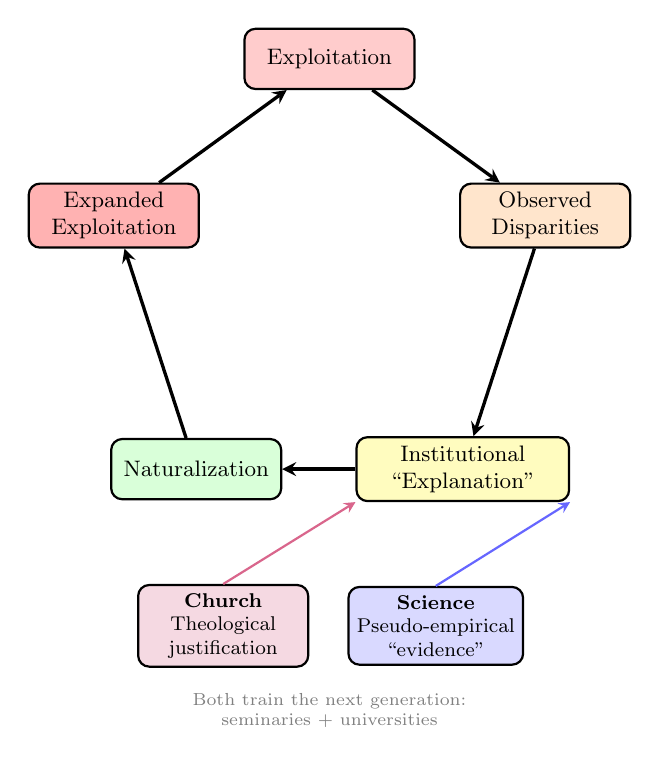
\begin{tikzpicture}[
    node distance=2.2cm,
    box/.style={draw, thick, rounded corners=4pt, minimum height=0.85cm, minimum width=2.4cm, align=center, font=\small},
    arr/.style={->, thick, >=stealth},
    scale=0.9, transform shape
]
    % Circular nodes
    \node[box, fill=red!20] (exploit) at (90:3.2) {Exploitation};
    \node[box, fill=orange!20] (dispar) at (18:3.2) {Observed\\Disparities};
    \node[box, fill=yellow!25, minimum width=3cm] (explain) at (-54:3.2) {Institutional\\``Explanation''};
    \node[box, fill=green!15] (natural) at (234:3.2) {Naturalization};
    \node[box, fill=red!30] (expand) at (162:3.2) {Expanded\\Exploitation};

    % Circular arrows
    \draw[arr, very thick] (exploit) -- (dispar);
    \draw[arr, very thick] (dispar) -- (explain);
    \draw[arr, very thick] (explain) -- (natural);
    \draw[arr, very thick] (natural) -- (expand);
    \draw[arr, very thick] (expand) -- (exploit);

    % Church and Science branches into "Explanation"
    \node[box, fill=purple!15, font=\footnotesize] (church) at (-1.5,-4.8) {\textbf{Church}\\Theological\\justification};
    \node[box, fill=blue!15, font=\footnotesize] (science) at (1.5,-4.8) {\textbf{Science}\\Pseudo-empirical\\``evidence''};

    \draw[arr, purple!60] (church.north) -- (explain.south west);
    \draw[arr, blue!60] (science.north) -- (explain.south east);

    % Education feedback
    \node[font=\scriptsize, align=center, gray] at (0,-6.0) {Both train the next generation:\\seminaries $+$ universities};
\end{tikzpicture}
\caption{\textbf{The Institutional Feedback Loop.} Exploitation produces disparities, which are ``explained'' by Church (theological justification) and Science (pseudo-empirical evidence) as inherent inferiority, naturalizing the hierarchy and licensing expanded exploitation. The cycle is self-perpetuating: each iteration generates new ``evidence'' that reinforces the ideological framework.}
\label{fig:feedback_loop}
\end{figure}

These parallel tracks of legitimation created a self-reinforcing institutional feedback loop (see Figure~\ref{fig:feedback_loop}).

\textbf{The Functional Necessity of Institutional Capture}

The Elite's capture of Church and Science was \textit{functionally necessary} for three reasons:

\begin{enumerate}
    \item \textbf{Moral legitimacy}: The implicit contract with the working class required a \textit{moral} justification for African exclusion; political imposition alone was insufficient. The Church provided this moral cover.
    
    \item \textbf{Intellectual legitimacy}: As education spread and Enlightenment values emphasized reason, exploitation required \textit{rational justification}. Science provided this intellectual cover.
    
    \item \textbf{Internalization}: For the system to be self-perpetuating, the dehumanization had to be \textit{internalized} as natural fact, not recognized as Elite strategy. When both God and Nature supposedly confirmed racial hierarchy, resistance seemed to oppose reality itself.
\end{enumerate}

The collaboration of Church and Science transformed racialization from a cynical political strategy into an apparently unchallengeable truth, backed by society's highest authorities on moral and empirical reality.

\subsection{The Counter-Signal: Anténor Firmin and the Empirical Demolition of Scientific Racism}
\label{sec:firmin_counter_signal}

The institutional feedback loop described above faced a direct challenge in 1885---the same year that Paul Topinard published his racialist \textit{Éléments d'anthropologie générale}. A Haitian lawyer, diplomat, and self-taught anthropologist named Joseph Auguste Anténor Firmin published \textit{De l'égalité des races humaines (anthropologie positive)} in Paris. It was the world's first sustained, book-length, \textit{empirically grounded} refutation of scientific racism \cite{firmin_legacy}. Its existence proves something structurally critical: the data the Elite's institutions were producing was analytically fraudulent, and it was possible to expose this fraud using the Elite's own methodology.

Firmin had been admitted to the Société d'Anthropologie de Paris (SAP) in 1884---the same institution founded by Paul Broca to systematize craniometric racial hierarchy. He was one of only three members of African descent. He was not encouraged to participate. He spent a year conducting a comprehensive positivist audit of the SAP's own data, bypassing the debate his colleagues would have dismissed \cite{firmin_legacy, drouinhans}.

What he found was devastating. The cranial measurements, brain volume charts, and anthropometric tables that were supposed to \textit{prove} racial hierarchy \textbf{wildly overlapped across populations}. There was no signal. Firmin concluded that the data was entirely \textbf{``anarchic''} and yielded no reliable indication of biological superiority \cite{firmin_legacy}. In the framework of this book, Firmin had done what any rigorous analyst must do when confronted with claimed empirical evidence: he stripped the ideological noise from the data and looked for the signal. The signal confirmed human equality. The noise was the extraction kernel's legitimation apparatus.

This is the precise mathematical argument this book makes about scientific racism: the Elite's institutions were running \textbf{confirmation-biased pattern-matching on pre-labeled data}. Firmin identified this before the terminology existed. His critique was so precisely defined that, as contemporary anthropologists note, he ``successfully undermined European anthropological practice as pure bias rather than empiricism'' \cite{firmin_legacy}---a finding that prefigures the Boasian revolution by forty years and anticipates modern critiques of racialized data collection by over a century.

\textbf{The Royer Contradiction: How Even Liberators Carry Enforced Priors.} Firmin demolished racial hierarchy with methodological precision. At the same time, he attacked Clémence Royer---the French feminist and first translator of Darwin into French---on the basis of her sex, ignoring the merits of her arguments. He asserted that problems of such complexity ``can be properly studied only by men'' \cite{drouinhans}. Firmin knew Royer's racial arguments were factually wrong. The grounds on which he dismissed her replicated the same structure he was dismantling: \textit{naturalized hierarchy based on an immutable biological characteristic}.

The structural observation this episode reveals is the following: the extraction kernel's partitioning logic had penetrated the epistemological infrastructure of 19th-century European intellectual life so thoroughly that even its most rigorous critics could dismantle one partition and operate entirely within another. The algorithm operates through locally dominant partitions, each kept beneath the threshold of critical scrutiny. No simultaneous enforcement of every prior is necessary. An analyst trained to see one axis of naturalized hierarchy is not automatically equipped to see the others---each prior reads as background reality before it is made the explicit object of analysis. This is the algorithm's deepest resilience property: it survives the dismantling of individual partitions because the dismantlers themselves are embedded in its remaining ones.

Firmin is the sharpest historical instance of this mechanism. In the language of this framework, he was operating his racial-liberation algorithm and simultaneously running the gendered version of the very Bayesian defense he was attacking. His prior on gender was as hard-coded as his colleagues' priors on race. In 1885 Paris, the gender partition was so deeply encoded as natural fact that even the man who had most precisely identified racial prior-enforcement could not perceive it operating in himself. The point is diagnostic: Firmin confirms the mechanism's general form and provides the clearest possible evidence precisely \textit{because} his racial analysis was so unusually rigorous. The more powerful his critique of one partition, the more visible his uncritical acceptance of another becomes.

\textbf{The System's Response.} The Société d'Anthropologie never reviewed \textit{De l'égalité des races humaines} in their \textit{Mémoires d'Anthropologie}---despite listing the book's publication without comment in October 1885 \cite{drouinhans}. The same institution that had enthusiastically circulated Gobineau's speculative racial hierarchies buried the only empirical refutation produced from within. The feedback loop's self-repair mechanism is visible here: \textbf{the algorithm identifies a threat to its legitimation architecture and applies institutional silence as a security patch}. Firmin's work would not receive full Anglophone recognition until its English translation in 2000---115 years after publication.

The structural lesson is permanent. The Elite's scientific institutions did not fail to notice Firmin's argument; they noticed it and suppressed it. The apparatus that was supposedly committed to empirical truth \textit{selectively enforced which empirical truths entered the canon}. This institutional censorship is the academic instantiation of the same pattern that criminalizes psychedelic research (Section~1.3.4), quarantines Haitian revolutionaries (Section~3.5), and algorithmically suppresses dissenting political content (Chapter~\ref{ch:recompile}). The system's response to a correct counter-signal is always the same: silence, marginalization, and the weaponization of institutional prestige against those who lack it. Firmin's deployment of the same analytical precision in the diplomatic domain---weaponizing the Elite's own legal conventions against its naval enforcement apparatus in 1891---is documented in Section~\ref{sec:firmin_protocol}.

\section{The Global Replication and the Export to America: Pirating the Source Code}

With the moral architecture authorized by the Church, the intellectual framework naturalized by Science, and the economic model proven spectacularly profitable in the Portuguese sugar colonies, the algorithm was ready for export. And export it did. Spanish and British colonies adopted and expanded the Portuguese model of racialization, each iteration refining the system: legal codes formalized racial categories (the \textit{one-drop rule}, blood quantum, \textit{limpieza de sangre}), religious institutions adapted theology to support racial hierarchy in new colonial contexts, and financial systems developed around slave-based wealth---insurance, banking, and eventually the securitization of enslaved human beings as mortgage collateral \cite{beckert, johnson}.

The algorithm spread wherever European colonialism reached, but its most consequential deployment occurred across the Atlantic. The transatlantic export of slave capitalism began with a direct theft of Portuguese inventory. No original American innovation produced it. In 1619, the English privateer \textit{White Lion} intercepted the Portuguese slave ship \textit{S\~{a}o Jo\~{a}o Bautista} and seized approximately 20 enslaved Africans, delivering them to the English colony at Point Comfort, Virginia. The first enslaved Africans in British North America were literally stolen from a Portuguese vessel---the algorithm's source code was \textit{pirated} from its original authors, not rewritten for the New World. The English colonists did not independently invent racialized slavery; they captured it, fully compiled, from the Portuguese system that had been running for over a century.

From this pirated origin, slave capitalism was systematically scaled across the American colonies, where it would become the economic foundation of the developing nation. The Implicit Contract crossed the Atlantic with the algorithm: poor European settlers in Virginia, the Carolinas, and the Caribbean were offered the same psychological wage ($\psi$) that the Portuguese peasantry had received---racial status in exchange for tolerating, and eventually enforcing, the extraction of the Out-group.

But the American deployment introduced a severe instability. In Portugal, the geographic separation between the Elite's plantations (on Atlantic islands and in Brazil) and the domestic working class meant the Implicit Contract was rarely tested. In the American colonies, enslaved Africans and indentured European servants \textit{labored side by side on the same plantations}, under the same brutal conditions. The ontological divide that Zurara had manufactured on paper was being stress-tested daily by the lived reality of shared suffering.

The algorithm, running on American wetware, was about to produce its first catastrophic system crash.

\begin{keyinsight}[Hardware Reading: The Initial Voltage Source]
At the circuit level, fifteenth-century Portugal was the first installation of a complete electrodynamic extraction grid. The Elite ($E$) functioned as the \textbf{control gate}: the architecture that directed the flow, distinct from the power supply. They set the system potential through the papal bulls \textit{Dum Diversas} and \textit{Romanus Pontifex}, establishing the extraction \textit{gradient} while the actual energy was supplied by the kinetic labor of the populations they subjugated. The African coast became the \textbf{source terminal} where charge ($+q$ for European, $-q$ for African) was first assigned by juridical decree independently of observed difference. The Middle Passage was the \textbf{initial current flow}---human beings as conduction medium---and the plantation was the \textbf{load} where extraction occurred. The psychological wage ($j\psi_s$) had not yet been invented; the system ran on naked violence and legal fiat. What Portugal engineered constituted the \textbf{circuit topology} itself: the five-node architecture (source, divider, current source, dielectric, sink) that every subsequent colonial power would replicate. The essential insight is parasitic: the Elite possessed no independent energy source sufficient to maintain the system. The entire architecture depended on continuous extraction from the source terminal.
\end{keyinsight}

\chapter{The Application: Bacon's Rebellion, the Buffer Class, and the Constitutional Patch (1676--1787)}
\label{ch:bacon}

\begin{tcolorbox}[colback=black!5, colframe=black!70, fonttitle=\bfseries\ttfamily, title=RUNTIME LOG: 1676--1787 (VIRGINIA COLONY $\rightarrow$ PHILADELPHIA)]
\ttfamily\small
\textbf{System Stress} ($\min$: class resistance): \textcolor{red}{\textbf{CRITICAL}} --- Cross-racial labor solidarity detected. Jamestown burning.\\
\textbf{Capital} ($\max$: extraction output): AT RISK --- Plantation economy destabilized by unified revolt.\\
\textbf{Interference State} ($\Phi_{\text{load}}$, proximity to $\tau$): TRANSITIONING --- coherence breach pre-patch, then rapid phase-loading via codified racial partition. Estimated $\Phi_{\text{load}} \in [0.15, 0.55]$; $\rho_{\tau}>1.00$ at crash, then $\rho_{\tau} \in [0.60, 0.75]$ post-patch.\\
\textbf{Active Patch}: Emergency recompile. Partitioning the poor\ldots\\
\textbf{Variables Loaded}: $E$, $O_{\text{racialized}}$, $I$.\\
\textbf{Variables Deployed This Cycle}: $I_{\text{buffer}}$ (Buffer Class), $F_{\text{enforce}}^{\text{proto}}$ (Proto-Enforcement Class---$I_{\text{buffer}}$ deputized to police racial boundary), $P_{\text{uppet}}^{\text{v1.0}}$ (Puppet Class---prototype), $W = j\psi_s$ (formalized).\\
\textbf{Executing Function}: Codify ``Whiteness.'' Weaponize the Implicit Contract into explicit law. Draft constitutional front-end.\\
\textbf{Result}: \textbf{[POLICY]} Virginia Slave Codes (1705) partition the working class and deputize $I_{\text{buffer}}$ as racial enforcers. \textbf{[POLICY]} Three-Fifths Compromise (1787) embeds extraction into federal architecture. \textbf{[POLICY]} Constitutional front-end/back-end separation prototypes $P_{\text{uppet}}$. $\min$ variable temporarily stabilized.
\end{tcolorbox}

\medskip

The two-variable system ($E$ and $O_{\text{racialized}}$) proved fatally unstable. In the American colonies, the Elite initially failed to implement the Portuguese code strictly. The result was the most dangerous event in Elite history: a unified working class that nearly destroyed them. This chapter is the first full application of the vector model from Chapters~\ref{ch:redefining}--\ref{ch:portugal} to a major system crash: it traces the emergency response---the invention of the Buffer Class ($I_{\text{buffer}}$), the formalization of $\psi$, and the constitutional patch that separated the Elite's front-end from their back-end---and shows how the invariant $\Delta\max = 0$ was preserved throughout: concessions that stabilized $I_{\text{buffer}}$ were funded through deeper extraction from $O_{\text{racialized}}$, not by any reduction in $E$'s own share (see the gloss on $\Delta\max = 0$ in Chapter~\ref{ch:redefining}).

Bacon's Rebellion exposes the virus's replication problem. A two-variable extraction system could seize labor, but it could not reliably colonize the mind of the poor European worker who shared the field, hunger, and violence of the enslaved African. The invention of whiteness solved that host-level failure. It gave the Buffer Class a psychological wage and a perception filter that recoded the person beside them as the dangerous Out-group whose containment proved membership in the protected class, displacing the prior perception of a co-exploited worker.

\section{The Application: Bacon's Rebellion and the Partition of the Poor (1676)}
In the American colonies, the Elite initially failed to implement this code strictly. The ``proto-working class'' was a mix of European indentured servants ($L_{white}$) and enslaved Africans ($L_{black}$). Because they shared the same oppressive conditions, the Portuguese distinction didn't stop them from seeing each other as allies.

The quantitative evidence for this shared condition is stark. Between 300,000 and 500,000 British and Irish people were shipped to the colonies as indentured servants over roughly 150 years---many of them involuntarily. Ship records listed them alongside livestock and supplies, as \textit{cargo}. The mortality data mirrors the Middle Passage: approximately 30\% died on the Atlantic voyage; another 40\% died during the period of bondage. Children were kidnapped en masse---a single trafficker named William Thiene abducted 840 children from Britain in a single year. Women were used as breeders: if a servant bore a child, the child was ``bound to serve until at least age 21, ensuring planters had a next generation of free labor'' \cite{jordan2008}. Elizabeth Abbott, abducted from England, was whipped 500 times by her enslaver after repeated escape attempts and died from her injuries. Nobody was charged. Out of the shipment of 300 children she arrived with, only 12 survived more than two years.

These were not ``indentured servants'' in any meaningful contractual sense. As the historians Don Jordan and Michael Walsh documented in \textit{White Cargo}, the system was ``slavery in all but name''---and for many, the legal distinction between temporary and permanent bondage was fiction. Out of 5,000 servants arriving in one colony between 1670 and 1680, only 241 ever became landowners; approximately 3,500 died before completing their contracts. The Dutch trader David Pietersz de Vries observed English planters gambling away their servants at card games, ``treating human lives as poker chips.'' Colonial courts almost universally sided with planters on complaints of abuse; contracts could be extended on fabricated charges---breaking a tool, talking back, falling ill.

White indentured servitude was not ``just as bad'' as African chattel slavery, particularly after the racial codes formalized. The operative point is that \textit{before} the racial partition, the Elite's extraction algorithm operated on a class basis across both populations. White servants and Black enslaved people shared the same fields, the same brutality, the same mortality rates---and above all, the same \textit{enemy}. Records document them running away together, sharing food, hiding in forests, and plotting rebellion. George Washington himself placed runaway advertisements in the \textit{Maryland Gazette} and the \textit{Virginia Gazette} offering identical rewards for the capture of both Black and white runaways---the same man, the same reward structure, the same system of human property management applied across racial lines.

This cross-racial solidarity was the system's existential vulnerability. It led to the system crash of \textbf{Bacon's Rebellion (1676)}. The united Labor Class ($L_{white} \cup L_{black}$) burned Jamestown to the ground, proving that:

\begin{equation}\label{eq:3.1-bacon-solidarity-condition}
\text{If} \quad (L_{white} + L_{black}) > E \quad \rightarrow \quad \text{Revolution}
\end{equation}

\section{The Pre-Compilation Patches: Prototyping the Racial Partition (1640--1691)}

The 1705 Slave Codes were the culmination of a 65-year iterative compilation cycle in which the Elite tested, debugged, and incrementally deployed the racial partition through a sequence of judicial decisions and statutes---each one closing a specific loophole in the extraction kernel. No single legislative session produced them.

\subsection{The Gendered Baseline: Regulatory Control and Reproductive Deviance}

To fundamentally understand the modern criminalization of pregnancy outcomes, we must establish the historical baseline of state-sanctioned violence against women in the United States and its preceding colonies. The earliest documented execution of a woman in the American colonies was that of \textbf{Jane Champion} in 1632 in the Virginia Colony. 

Among the most distinctly gendered crimes in early American legal history was the offense of \textbf{``concealing a birth,''} adopted beginning in 1696 to regulate female sexuality and punish women who gave birth out of wedlock. These early protocols established that the state's regulatory control over the female body would be enforced through the ultimate penalty from the very beginning of the colonial project. A comprehensive analysis of this parallel axis of oppression---the gendered axis ($O_{\text{gendered}}$)---is provided in Chapter~\ref{ch:gendered}.

\subsection{John Punch (1640): The First Racial Sentencing Disparity}

The earliest documented instance of the racial partition operating as law occurred 36 years \textit{before} Bacon's Rebellion. In 1640, three indentured servants---John Punch, a Black man; a Scotsman; and a Dutchman---ran away together from their Virginia enslaver. All three were recaptured. The court sentenced the two white servants to four additional years of indenture. John Punch was sentenced to servitude \textit{for life}.

Same crime. Same act of cross-racial solidarity. Racially bifurcated punishment. The Virginia court, in a single judicial act, instantiated the $I_{\text{buffer}}$ / $O_{\text{racialized}}$ partition: the white men's punishment was temporal (additional years within the existing system); the Black man's punishment was categorical (permanent exclusion from the system of eventual freedom). The court articulated no racial theory, cited no scripture or science, and simply treated the same behavior differently based on phenotype---the first recorded instance of the function $O_{\text{racialized}} = f(\text{phenotype})$ operating in American law.

The Punch case is analytically significant for a second reason: it documents interracial solidarity \textit{in action}---three workers of different races running away together---and reveals the judicial system's response, which destroyed the conditions that made solidarity possible; the solidarity itself went unpunished. The system's answer to cross-racial cooperation was legal differentiation first, ideological justification second. The causal arrow of the framework---Elite economic interests $\rightarrow$ systemic racialization $\rightarrow$ interpersonal prejudice---is visible here in its earliest American instantiation.

\subsection{The Codification Sequence (1662--1669): Compiling the Racial Kernel}

Over the next three decades, the Virginia and Maryland legislatures iteratively closed the loopholes in the extraction kernel through a sequence of statutes, each one hardening the racial partition along a specific axis:

\begin{enumerate}
    \item \textbf{1662 --- \textit{Partus sequitur ventrem} (Virginia):} Hereditary slavery codified. A child's legal status now followed the \textit{mother}, not the father---closing the loophole by which children of enslaved women and white men might claim free status through paternal lineage. The rule operated as \textit{supply-chain optimization}; moral principle was not its basis. By tying enslaved status to the maternal line, the Elite ensured that the rape of enslaved women by white enslavers \textit{expanded} the enslaved labor supply, preventing dilution.

    \item \textbf{1664 --- Maryland Slave Law:} All persons of African descent declared slaves \textit{for life}. This closed the temporal boundary: where indentured servitude had a contractual endpoint, the Maryland statute eliminated it entirely for Black people, making the condition permanent and irrevocable regardless of individual circumstance.

    \item \textbf{1669 --- ``An Act About the Casual Killing of Slaves'' (Virginia):} If an enslaved person died ``during correction,'' the death would not be treated as a felony. This statute removed the last moral constraint on the extraction kernel: the prohibition on killing. The Elite explicitly exempted themselves from homicide liability when the victim was enslaved property---a legal distinction never codified for white servants, no matter how brutally they were treated. The law's internal logic was revealing: it assumed ``no man would destroy his own property willingly,'' thereby defining the enslaved person as a capital asset whose destruction was merely an imprudent business decision.
\end{enumerate}

Each statute corresponds to a specific constraint on the extraction kernel:
\begin{itemize}
    \item 1662 closes the \textbf{boundary leak}: heritable enslavement ensures a permanent, self-reproducing labor supply.
    \item 1664 closes the \textbf{temporal leak}: life servitude eliminates the contractual endpoint that still connected Black bondage to the indentured servitude model.
    \item 1669 removes the \textbf{enforcement liability}: $F_{\text{enforce}}$ (here, the slaveholding class itself) can kill without legal consequence.
\end{itemize}

Together, these three statutes compiled the racial kernel before 1705 formalized the user interface. The 1705 Slave Codes were a \textit{release version}---the public-facing codification of a system that had been iteratively debugged through judicial and legislative patches for 65 years.

\subsection{The Boundary Enforcement Act (1691): Criminalizing the Crossing}

With the racial categories being assembled through the 1662--1669 sequence, the Elite faced a structural anxiety: the categories were inherently \textit{unstable}. Cross-racial reproduction would produce ambiguous-status children who blurred the partition line. If the boundary between $I_{\text{buffer}}$ and $O_{\text{racialized}}$ could not be policed at the reproductive level, the entire architecture was vulnerable to dissolution through miscegenation.

In 1691, Virginia enacted a law that criminalized the crossing itself: a white woman who bore a child with a Black man would have \textit{five years added to her indenture}, and the child would be \textit{indentured for thirty years}. The statute functioned as a \textbf{boundary enforcement mechanism}; its purpose was to maintain the racial partition. Sexual behavior was regulated only insofar as it threatened that partition. The statute maintained:

\begin{equation}\label{eq:3.2-boundary-enforcement-1691}
I_{\text{buffer}} \cap O_{\text{racialized}} = \emptyset
\end{equation}

The\footnote{This equation is classified as Tier~3 (ordinal/structural); the set-disjointness condition $I_{\text{buffer}} \cap O_{\text{racialized}} = \emptyset$ is a structural claim validated by the 1691 Virginia anti-miscegenation statute and its 276-year legal lineage through \textit{Loving v.\ Virginia} (1967) \cite{loving_v_virginia_record_1967}. See the Empirical Methodology chapter (p.~\pageref{ch:empirical_methodology}) and Appendix~\ref{app:empirical_index}.} 30-year indenture for a child born of that crossing is analytically revealing: the child was neither fully enslaved (the father's status did not automatically apply) nor fully free (the mother's ``transgression'' of the racial boundary imposed a punitive condition). The system treated boundary-blurring as a vulnerability requiring punishment-as-deterrent---anticipating the ``one-drop rule'' and all subsequent racial purity statutes by over a century.

The 1691 law demonstrates that the Elite recognized from the beginning that the racial partition was \textit{artificial} and required \textit{coercive maintenance}. A natural category does not need a law criminalizing its violation. The very existence of the boundary enforcement statute proves that the partition was engineered---and that the Elite knew it was fragile. This structural anxiety---the fear that the racial wall could be dissolved through human solidarity---is the same anxiety that would drive the Black Codes, the anti-miscegenation laws, Jim Crow, and the modern carceral state. The system has been repairing the same artificial partition for over 350 years.

\paragraph{The 276-Year Arc: From the 1691 Statute to \textit{Loving v.\ Virginia} (1967).}
The 1691 Virginia boundary enforcement act was not a colonial artifact that faded with colonial governance. It was a legal lineage. Virginia's 1924 Racial Integrity Act---a direct statutory descendant of the 1691 law---was the instrument under which Mildred and Richard Loving were arrested in 1958, convicted in 1959, and sentenced to one year in prison (suspended on the condition that they leave Virginia for twenty-five years). Mildred Loving was a Black woman. Richard Loving was a white man. They had married in Washington, D.C.---a jurisdiction without the prohibition---and returned to Caroline County, Virginia to live as husband and wife. The state treated their domestic arrangement as a felony. In 1965, with their case still on appeal, the Circuit Court of Caroline County denied their motion to vacate. The presiding judge, Leon Bazile, wrote an opinion whose text is now publicly accessible through the Internet Archive's 2026 Supreme Court records release \cite{bazile_opinion_1965, ia_scotus_briefs_2026}:

\begin{quotation}
``Almighty God created the races white, black, yellow, malay and red, and he placed them on separate continents. And but for the interference with his arrangement there would be no cause for such marriages. The fact that he separated the races shows that he did not intend for the races to mix.''
\end{quotation}

The framework's classification of this text is unambiguous. Judge Bazile is producing Component~3 ideological justification: the theological overlay applied to a political-economic substrate. The 1691 statute exists for Buffer-Class-maintenance reasons---equation~\ref{eq:3.2-boundary-enforcement-1691} must hold ($I_{\text{buffer}} \cap O_{\text{racialized}} = \emptyset$) because cross-racial kinship networks dissolve the partition that the entire extraction architecture depends upon. Bazile's deity is invoked to sanctify a Bacon's-Rebellion-era security patch. What the \textit{Loving} record makes uniquely visible is the self-documentation of Component~3 by an officer of the state, in an official judicial opinion, 263 years after the original statute: the claim that the partition is divinely ordained is the system's own witness against itself. A structure that cites God to justify its maintenance has no stable justification in nature, science, or human solidarity; each of those would run the other direction.

The Supreme Court unanimously reversed in \textit{Loving v.\ Virginia}, 388 U.S.\ 1 (1967) \cite{loving_v_virginia_record_1967}, striking the Racial Integrity Act as unconstitutional under both the Equal Protection and Due Process Clauses of the Fourteenth Amendment. Chief Justice Warren, writing for a unanimous Court, named the system's logic with unusual directness: ``There is patently no legitimate overriding purpose independent of invidious racial discrimination which justifies this classification. The fact that Virginia prohibits only interracial marriages involving white persons demonstrates that the racial classifications must stand on their own justification, as measures designed to maintain \textbf{White Supremacy}.''\footnote{\textit{Loving v.\ Virginia}, 388 U.S.\ 1, 11 (1967) (Warren, C.J.) (emphasis added). The Bazile--Warren collision is the framework in miniature: a state judge invoking God in 1965 to justify a 1691 security patch; a Chief Justice in 1967 characterizing that patch accurately as ``White Supremacy.'' Both texts are now publicly accessible in the Internet Archive's 2026 SCOTUS records release \cite{ia_scotus_briefs_2026}. The framework requires only that its readers read them.} This was \textit{Marbury} exercised: a court voiding a legislative act that failed constitutional scrutiny. The framework's structural prediction holds: voiding the anti-miscegenation law removed one instance of the boundary enforcement mechanism while the surrounding architecture---criminal sentencing disparities, housing segregation, employment discrimination, differential enforcement---remained entirely intact. The kernel does not require any single statute; it requires the partition. When one enforcement mechanism is struck, the others absorb its function. \textit{Loving} is proof of concept: the Out-group's strategic litigation can edit the source code. The extraction kernel's adaptive resilience is that the source code is larger than any single edit.

\section{The Patch: The Explicit Codification of ``Whiteness'' (1705)}
As established in Chapter~\ref{ch:portugal}, the concept of racial whiteness was \textit{created} in 15th-century Portugal through the Implicit Contract---the unwritten agreement that divided the population into a privileged In-group ($I$) and an exploited Out-group ($O_{\text{racialized}}$), compensating the former with the psychological wage ($\psi$). But in Portugal, this boundary remained implicit: informal, unwritten, and enforced by custom rather than statute.

To prevent a recurrence of the cross-racial solidarity that had nearly toppled them, the Virginian Elite \textbf{explicitly defined and legally codified} whiteness. The Portuguese had originated the concept; the Virginians hardened it into law. They enacted the \textbf{Virginia Slave Codes of 1705}, which hardened the Portuguese implicit boundary into an explicit legal wall between the two groups \cite{allen, kendi}.

\begin{enumerate}
    \item \textbf{The Partition:} They assigned $L_{white}$ to a new category: "White."
    \item \textbf{The Bribe:} They gave the poor whites the psychological wage $\psi$ (Chapter~\ref{ch:portugal})---the right to police the Black population, the right to bear arms, and immunity from chattel slavery.
\end{enumerate}

This was the definitive move of the American algorithm: It used "Race" to destroy "Class." It recruited the poor white population to act as the \textbf{Buffer Class}, protecting the Elite from the very people they should have been allied with.\footnote{Equation~\ref{eq:3.3-race-destroys-class} is classified as Tier~3 (ordinal/structural); the structural transition from poor white laborer to Elite defender is an ordinal claim validated by the documented sequence from Bacon's Rebellion (1676) to the Virginia Slave Codes (1705). See the anchor case study on p.~\pageref{cs:bacons_rebellion} and the Empirical Methodology chapter (p.~\pageref{ch:empirical_methodology}).}

\begin{equation}\label{eq:3.3-race-destroys-class}
\text{Buffer Created:} \quad I_{poor} \rightarrow \text{Defender of } E
\end{equation}

\section{Formalizing the Buffer Class ($I_{\text{buffer}}$): From Implicit In-group to Weaponized Partition}

In Chapter~\ref{ch:portugal}, we introduced the In-group ($I$) as the automatic byproduct of the Portuguese Implicit Contract---the working-class population compensated with the psychological wage ($\psi$) in exchange for tolerating the extraction of the Out-group. But the In-group as it existed in 15th-century Portugal was an \textit{implicit} variable: the contract was unwritten, the racial boundary was informal, and significantly, the partition had no legal enforcement mechanism in the American colonies.

Bacon's Rebellion proved that an implicit In-group left the system vulnerable. The invention of ``Whiteness'' in 1705 was the \textit{formalization} of this variable---the upgrade from a passive In-group to an actively \textbf{weaponized Buffer Class}. The Elite's emergency patch was to harden the racial boundary with legal force, transforming the In-group from a loosely defined beneficiary of the psychological wage into a legally codified human shield between $E$ and $O_{\text{racialized}}$. We now formalize this upgraded tier.

\begin{definition}[The Buffer Class]
\textbf{The Buffer Class ($I_{\text{buffer}}$):} The remaining working-class In-group. They produce the economic reserves and provide the ideological cover required to legitimize the state, pacified by the suppression allocation ($\psi = \psi_s + \psi_m$) and the illusion of democratic agency. Building on W.E.B.\ Du~Bois's formulation of the ``\textbf{public and psychological wage}'' \cite{dubois}---his term capturing both the symbolic status benefits and the public infrastructure advantages (better schools, police protection, court leniency) granted to white workers---this framework formalizes $\psi$ as a two-mode variable and traces its operation four centuries before Du Bois's Reconstruction-era analysis:

\begin{itemize}
    \item $\psi_s(t)$: \textbf{status wage}---the non-material guarantee of ontological superiority and racial privilege (Du Bois's ``titles of courtesy,'' hierarchy over $O_{\text{racialized}}$). Default mode. Costs $E$ nothing to dispense.
    \item $\psi_m(t) \geq 0$: \textbf{material wage}---calibrated material concession (land grants, welfare benefits, subsidized homeownership) deployed only when $M(t) \to \tau$. Invariant: $\psi_m(t)$ is sourced from \textit{increased $O_{\text{racialized}}$ extraction}, never from reduced Elite share. $\Delta\max = 0$ is preserved.
\end{itemize}
\end{definition}

The foundational inequality of the system upgrades to three tiers:
\begin{equation}\label{eq:3.4-three-tier-post-bacon}
\text{Benefit}(E) \gg \text{Benefit}(I_{\text{buffer}}) > \text{Benefit}(O_{\text{racialized}})
\end{equation}

where\footnote{This equation is classified as Tier~3 (ordinal/structural); the ordinal inequality is confirmed by the documented wealth and legal-status distributions in colonial Virginia 1705--1776---planters' estates versus indentured servant wages versus enslaved persons' legal non-personhood. See the Empirical Methodology chapter (p.~\pageref{ch:empirical_methodology}) and Appendix~\ref{app:empirical_index}.} $\text{Benefit}(I_{\text{buffer}})$ consists of the suppression allocation $\psi$ rather than Elite-level extraction, and $\text{Benefit}(E)$ reflects the material wealth extracted from all tiers below.

The suppression allocation $\psi$ is a \textit{designed feature} of the system. In its default mode ($\psi_m = 0$), $E$ pacifies $I_{\text{buffer}}$ without surrendering a single unit of extraction: racial status, legal privileges over $O_{\text{racialized}}$, and the right to police the racial boundary cost the Elite nothing material. When kinetic threat demands escalation ($\psi_m > 0$), the Elite fund the material concession by deepening $O_{\text{racialized}}$ extraction---ensuring the buffer class's material gains are always paid for by the Out-group, never by $E$. This makes $\psi$ the key variable in the system's minimization of class resistance. The system thus produces a paradox: $I_{\text{buffer}}$ defends a hierarchy that materially harms them, because the suppression allocation creates the \textit{perception} of shared interest with $E$ and the \textit{perception} of threat from $O_{\text{racialized}}$. Both perceptions serve $E$'s extraction objectives.

\subsubsection{The Autonomy Wage: The Currency of Complicity}

We must refine our understanding of the psychological wage ($\psi$). Beyond the passive comfort of ``status superiority,'' it is actively experienced as \textbf{Autonomy Sovereignty} ($\psi_{\text{autonomy}}$).

The Buffer Class is compensated with the visceral feeling that \textit{their} autonomy is a universal, unassailable right, while the Out-group's autonomy is a conditional privilege granted (and revocable) by the state. This explains the intense, seemingly disproportionate rage exhibited by the Buffer Class when Out-group rights are advanced. 

Because the Buffer Class possesses little actual material capital (which is hoarded by $E$), their primary ``wealth'' is this Autonomy Wage. Therefore, they perceive any gain in Out-group autonomy as a direct, zero-sum theft of their own sovereign status; the possibility of equality does not enter their calculation. When the system grants $O_{\text{racialized}}$ the right to vote, or the right to exist in previously segregated spaces, $I_{\text{buffer}}$ experiences this mathematically as a wage cut. This guarantees that $I_{\text{buffer}}$ will viciously police the boundary on behalf of $E$, ensuring the $\min$ variable (resistance to the Elite) remains near zero.

\subsection{The Necessary Condition Theorem: Who Actually Needed Whom}
\label{sec:necessary_condition}

\chapter{The Constitutional Kernel: Firmware, Bootloader, and Power Supply (1787--1791)}
\label{ch:constitutional}

This chapter treats the founding documents as engineering artifacts. The Constitution is the bootloader. The \textit{Federalist Papers} are design whitepapers. The Bill of Rights is a security patch bundle. The slavery provisions are extraction algorithms embedded at the kernel level. Hamilton's financial architecture is the power-supply specification. It reads the Framers' own words---particularly Madison's Convention notes and the \textit{Federalist} essays---as technical documents in which the authors explicitly discuss failure modes, redundancy, load balancing, and threat surfaces with the precision of control-system theorists.

\section{The Constitution as BIOS: From Colonial Patch to National Bootloader}

In the computing stack developed in Chapter~\ref{ch:redefining}, the firmware layer translates abstract ideology into machine-readable instructions for the hardware. The Constitution performs exactly this function. It does not extract wealth directly; no clause in Article~I orders the seizure of labor or property from $O_{\text{racialized}}$. Instead, it establishes the \textbf{instruction set} that makes such extraction executable by subsequent legislatures and courts.

The distinction between the Declaration of Independence and the Constitution clarifies this layer separation. The Declaration is user-interface text: it displays egalitarian principles to the population, generating legitimacy and compliance sentiment. The Constitution is kernel code: it determines which processes can access which resources, how memory (territory, jurisdiction, representation) is allocated, and what permissions (taxation, commerce, war, enforcement) each branch possesses. A user-level program (a citizen petition, a state statute, a jury verdict) cannot alter kernel permissions without a specific amendment protocol---which the Framers set at a threshold high enough to prevent any popular majority from recompiling the system without Elite-aligned supermajorities.

The electrodynamic mapping is precise. The Constitution establishes the \textbf{circuit topology}: it wires the branches together, specifies the conductivity between federal and state nodes, and installs the ground plane (federal supremacy) that ensures all local currents ultimately reference the national voltage source. Without this topology, the colonial extraction patches examined in Chapter~\ref{ch:bacon} could not scale. The 1705 Virginia Slave Codes were effective within a single county. The Fugitive Slave Clause of Article~IV, Section~2---the same extraction logic elevated to federal mandate---was effective across the entire continent.

\subsection{The Three-Fifths Compromise: Algorithmic Optimization}

The most explicit extraction algorithm embedded in the constitutional kernel is the Three-Fifths Compromise (Article~I, Section~2). The Framers faced an optimization problem: how to maximize the political power of the slave-holding Elite without granting personhood to the enslaved population that generated that power.

Classifying the compromise as a moral concession misidentifies its function. It is a \textbf{mathematical subroutine}. Each enslaved person counted as three-fifths of a free person for purposes of congressional apportionment and direct taxation. This yielded a dual extraction:

\begin{enumerate}
    \item \textbf{Political amplification}: Slave states received disproportionate representation in the House and the Electoral College, powered by a population they explicitly denied the right to vote, speak, or assemble. The Out-group's biological existence was converted into political capital for the Elite.
    \item \textbf{Tax minimization}: The same three-fifths ratio applied to direct taxation, limiting the federal revenue that could be extracted from slave property. The Elite captured representational surplus while minimizing fiscal liability.
\end{enumerate}

This is the \textbf{Demographic Paradox} in its original compiled form: $O_{\text{racialized}}$ is simultaneously excluded from civic personhood and weaponized as a mathematical input to amplify Elite power. The algorithm would later be replicated in the prison-industrial complex, where incarcerated populations count toward census apportionment and economic development grants while being denied suffrage---the same three-fifths logic operating through a different interface.

\subsection{The Fugitive Slave Clause: Remote Procedure Call}

Article~IV, Section~2 requires that ``no Person held to Service or Labour in one State, under the Laws thereof, escaping into another, shall, in Consequence of any Law or Regulation therein, be discharged from such Service or Labour, but shall be delivered up on Claim of the Party to whom such Service or Labour may be due.''

In systems-engineering terms, this is a \textbf{remote procedure call} (RPC). The extraction kernel executes in Virginia, but if the target resource (the enslaved person) migrates to Pennsylvania, the Virginia process can invoke federal protocol to force the Pennsylvania node to return the resource. The clause overrides any local statute that might terminate the extraction process. It nationalizes the enforcement perimeter, ensuring that geographical escape cannot interrupt the algorithm.

The Fugitive Slave Act of 1790, passed by the First Congress, compiled this RPC into executable statute. The 1850 Fugitive Slave Act upgraded it with federal marshals, citizen deputization, and criminal penalties for non-compliance---an escalation pattern that demonstrates the kernel's increasing enforcement priority as abolitionist threats rose. Each iteration increased the coercive bandwidth of the RPC without altering its core logic.

\subsection{The Slave Trade Moratorium: Depreciation Scheduling}

Article~I, Section~9 prohibits Congress from banning the importation of enslaved persons before 1808. The Framers set a twenty-year sunset for the trade. Immediate abolition would have destabilized the economic load; the deprecation schedule allowed the existing extraction infrastructure to amortize its capital investments while signaling that future kernel versions would rely on domestic reproduction (the ``natural increase'' of the enslaved population), ending importation. The 1808 ban completed the deprecation schedule that the Framers had written into the source code in 1787. Humanitarian reform was not its operating logic.

\section{The Federalist Papers as Design Whitepapers}

The eighty-five essays published under the pseudonym ``Publius'' during 1787--1788 constitute the most detailed systems-engineering documentation ever produced for a national operating system. Hamilton, Madison, and Jay wrote \textbf{threat assessments, redundancy specifications, and load-balancing algorithms} designed to persuade skeptical state ratifiers that the proposed kernel would survive documented failure modes.

\subsection{Federalist No.~10: The Interference Engine Specification}

James Madison's \textit{Federalist No.~10} is the foundational control-system theory document of the American extraction architecture. Madison identifies the core threat to Elite stability with mathematical clarity: ``a majority\ldots united by a common impulse or passion\ldots\ adverse to the rights of other citizens\ldots or to the permanent and aggregate interests of the community.'' In the framework's vocabulary, this is the coherence threat $M(t) \rightarrow \tau$.

Madison's solution is to \textbf{manage} factions: ``extend the sphere, and you take in a greater variety of parties and interests; you make it less probable that a majority of the whole will have a common motive to invade the rights of other citizens.'' This is the Interference Engine in its original specification. By increasing the dimensionality of the identity space---adding regional, religious, occupational, and property-based axes to the political spectrum---Madison ensures that any potential class-majority wave is scattered into non-coherent components before it can achieve constructive amplitude.

The electrodynamic mapping is exact. Madison's ``greater variety of parties and interests'' corresponds to the superposition of magnetic fields $B_k$ across multiple identity axes. Each faction becomes a charged particle in a multi-dimensional $B$-field. A majority attempting vertical mobility (demanding material concessions from $E$) is deflected into horizontal collision with other factions. The Buffer Class fights the Out-group along racial lines; the agricultural sector fights the mercantile sector along regional lines; creditors fight debtors along class lines. The time-averaged displacement along the material axis approaches zero. The Engine executes the same function that Chapter~\ref{ch:redefining} formalizes as the phase-loading architecture: $\Phi_{\text{load}}(t) = 1 - |(1/N) \sum e^{i\Phi_j}|$.

Madison did not discover this mechanism accidentally. He observed it in the state legislatures of the 1780s, where debtor majorities had passed paper-money laws and property seizures that threatened creditor capital. His design response was to scale the system up: a large republic contains so many competing interests that no single majority can form without Elite-aligned intermediaries (the Puppet Class) brokering coalitions. The \textit{Federalist No.~10} architecture is the deliberate engineering of destructive interference.

\subsection{Federalist No.~51: Separation of Powers as Redundancy Engineering}

Madison's \textit{Federalist No.~51} specifies the \textbf{failover architecture} that prevents any single branch from defecting from the extraction kernel. ``Ambition must be made to counteract ambition.'' Each branch receives distinct permissions (legislative, executive, judicial) and each is populated by actors with overlapping class interests but competing institutional loyalties.

The framework classifies these mechanisms as \textbf{redundancy engineering}: failover architecture that prevents any single branch from defecting from the extraction kernel. A system with a single point of failure (a monarch, a populist legislature) can be captured by a coherence threat that breaches that single node. A system with three mutually checking branches requires the coherence threat to capture all three simultaneously---a statistical improbability when each branch is filtered through different selection mechanisms (districted election, Electoral College, presidential nomination with senatorial confirmation).

These mechanisms empower one Elite-filtered node to block another, leaving popular majorities without a corresponding override. The President can veto legislation; the Senate can block appointments; the courts can void statutes. The architecture ensures that $P_{\text{uppet}}$ cannot be captured by $O_{\text{racialized}}$ or by a cross-class coalition because the three branches are designed to neutralize each other unless all three align---which requires the same capital-backed candidate pool to control each.

\subsection{Federalist No.~78: Judicial Review as Conditional Circuit Breaker}

Alexander Hamilton's \textit{Federalist No.~78} describes the judiciary as the ``least dangerous'' branch because it controls ``neither the sword nor the purse.'' It can issue rulings but cannot enforce them. In circuit terms, the judiciary is a \textbf{voltage sensor}, not a current source. It measures whether legislative output exceeds constitutional bounds but lacks the $F_{\text{enforce}}$ capacity to execute its own judgments.

The framework formalizes this as a \textbf{conditional circuit breaker}. The courts can trip (void a statute) only when the political branches permit the trip to stand. \textit{Marbury v.~Madison} (1803) established the trip mechanism; the subsequent history of judicial abdication---particularly the refusal to void racial extraction statutes during Jim Crow---establishes the conditionality. The breaker trips when Elite capital is not threatened. It fails to trip when Elite capital depends on the circuit it would otherwise break.

Hamilton understood this precisely. He wrote that judicial review would protect against ``occasional ill humors in the society''---populist spasms that might produce redistributionist legislation. The breaker was designed to interrupt majority impulses while leaving Elite prerogatives intact. Its subsequent deployment confirms the design intent: judicial review voided New Deal labor protections, civil rights remedial statutes, and campaign-finance restrictions far more reliably than it voided slavery, segregation, or corporate extraction.

\section{The Bill of Rights as Security Patch Bundle}

The ten amendments ratified in 1791 function as \textbf{security patches}---targeted fixes for specific failure modes that the Framers had observed in British and colonial governance.

\begin{itemize}
    \item \textbf{First Amendment (Religion, Speech, Press, Assembly, Petition)}: Patches the sectarian warfare that had destabilized Europe for centuries. By prohibiting a state religion, the kernel prevents theocratic factions from capturing $P_{\text{uppet}}$ and waging religious wars that would divert extraction energy. Free speech and assembly function as \textbf{pressure-release valves} that allow thermal dissipation (protest, pamphleteering) without permitting the pressure to reach the threshold of kinetic system breach.
    
    \item \textbf{Second Amendment (Arms)}: The kinetic guarantee and anti-tyranny protocol, analyzed in full in Chapter~\ref{ch:kinetic}. The Framers installed an armed populace as a distributed threat surface against tyrannical capture---while simultaneously restricting the recognition domain to the propertied white class that composed $I_{\text{buffer}}$. The amendment is a security module with an explicit access-control list.
    
    \item \textbf{Third Amendment (Quartering of Troops)}: Patches a specific colonial grievance (British troop billeting) that had generated localized resistance. It prevents $F_{\text{enforce}}$ from consuming $I_{\text{buffer}}$ housing resources without compensation, preserving the psychological wage by respecting Buffer Class property boundaries.
    
    \item \textbf{Fourth Amendment (Search and Seizure)}: Establishes procedural impedance for $F_{\text{enforce}}$. The warrant requirement inserts bureaucratic resistance ($R$) into the enforcement circuit, calibrated to protect $I_{\text{buffer}}$ property while remaining permeable to Out-group enclosure. The historical record confirms this differential impedance: warrant requirements were enforced against white property owners and routinely waived for Black, Indigenous, and poor populations.
    
    \item \textbf{Fifth--Eighth Amendments (Due Process, Speedy Trial, Jury, Cruel and Unusual Punishment)}: Procedural patches that slow the enforcement pipeline, require evidentiary standards, and limit visible brutality. These are \textbf{legitimacy-preservation modules}. They prevent extraction from becoming so overt that it triggers legitimacy-collapse ($C_{\text{legitimacy}} \rightarrow \tau$). The Eighth Amendment's prohibition on cruel and unusual punishment is particularly precise: it prohibits \textit{cruel and unusual} punishment---punishment that exceeds the population's normalized threshold for visible state violence.
    
    \item \textbf{Tenth Amendment (State Sovereignty)}: The \textbf{sandbox patch}. It reserves non-delegated powers to the states, creating jurisdictional compartments where extraction algorithms can run in localized environments without federal interference. This patch enables the Jim Crow operating system (1877--1964): state-level segregation, disenfranchisement, and labor extraction that the federal kernel does not interrupt because the Tenth Amendment places those functions outside federal enumerated powers.
\end{itemize}

The Bill of Rights is a \textbf{targeted patch bundle} installed by systems engineers who had observed that unregulated extraction generates resistance, and that resistance threatens kernel stability. Each amendment addresses a specific historical failure mode; each preserves extraction by managing its side effects.

\section{Hamilton's Financial Architecture: The Power Supply}

The constitutional kernel required a voltage source. Alexander Hamilton's financial program (1790--1791) supplied it. The Report on Public Credit, the Bank of the United States, and the federal excise tax established the \textbf{economic backend} that the constitutional front-end had been designed to protect.

Hamilton's assumption of state debts converted the Revolutionary War obligations of the states into federal Treasury bonds held by the creditor class---the same class that composed the Constitutional Convention's dominant faction. This accomplished three engineering objectives simultaneously:

\begin{enumerate}
    \item \textbf{Capital consolidation}: It centralized the nation's credit architecture in New York and Philadelphia, creating a single node through which all significant financial flows had to pass. The Bank of the United States functioned as a \textbf{central router}: it issued currency, managed government deposits, and extended credit to commercial enterprises. Control of the router meant control of the network.
    
    \item \textbf{Elite alignment}: By funding the bonds at face value, Hamilton transferred wealth from taxpayers (predominantly farmers and artisans) to speculators (predominantly urban merchants and bondholders). The operation was explicit: James Madison objected precisely because it rewarded speculators who had purchased depreciated paper from desperate veterans at pennies on the dollar. Hamilton's response was that the nation's credit required honoring the paper at face value---which happened to concentrate capital in the hands of the creditor Elite.
    
    \item \textbf{Federal enforcement capacity}: The excise tax on whiskey (1791) and the subsequent military suppression of the Whiskey Rebellion (1794) demonstrated that the federal kernel possessed both the revenue extraction mechanism and the coercive bandwidth to enforce it. The rebellion was a class-coherence threat: small farmers in western Pennsylvania resisted a tax that fell disproportionately on their cash crop while sparing eastern commercial capital. The federal response---13,000 troops, the largest domestic military deployment until the Civil War---proved that the new OS could process resistance through its enforcement pipeline.
\end{enumerate}

Hamilton's program is the \textbf{power-supply specification} for the constitutional circuit. It converts the nation's productive capacity into a centralized voltage source, routes that voltage through Elite-controlled financial institutions, and installs the enforcement architecture necessary to maintain the flow against localized resistance.

\section{The Framers as Systems Engineers: A Conclusion}

The evidence reads the Framers as \textbf{deliberate architects} who understood exactly what they were building. The sentimental reconstruction---idealists who failed to live up to their own principles---finds no support in the documents.

They understood that a large republic could manage factions by scattering them across multiple identity axes (\textit{Federalist No.~10}). They understood that separating powers prevented any single popular majority from capturing the state (\textit{Federalist No.~51}). They understood that judicial review could void legislation threatening Elite capital while preserving legislation enforcing extraction (\textit{Federalist No.~78}). They understood that the Three-Fifths Compromise would amplify their political power while denying personhood to the population that generated it. They understood that a national bank and federal debt assumption would concentrate financial power in their own class. They wrote all of this down.

The framework reads the Framers as engineers whose behavior aligned with their output. Hypocrisy implies a gap between stated belief and actual behavior, and that gap is absent here. They wrote the Declaration's egalitarian interface text because interfaces generate compliance. They wrote the Constitution's extraction kernel because kernels generate output. Both documents served the same system. The interface was the user-facing display; the kernel was the executable code. The user who mistakes the display for the code has misunderstood the architecture.

\begin{keyinsight}[Firmware Reading: The Constitutional BIOS]
The Constitution functions as a \textbf{bootloader}: the first code executed when the American operating system starts. It initializes the memory map (federalism), loads the drivers (branches of government), establishes the privilege levels (who can tax, who can enforce, who can judge), and embeds the extraction algorithms (Three-Fifths Compromise, Fugitive Slave Clause, Commerce Clause) as kernel-space modules that user-level programs cannot modify without supermajority access. The Bill of Rights is a patch bundle addressing known vulnerabilities. The \textit{Federalist Papers} are the design whitepapers. The founding generation were social engineers in the literal, technical sense: they diagnosed failure modes, specified redundancies, and compiled a national extraction architecture that has run for two centuries with only interface-level updates.
\end{keyinsight}
